% The Finite Element Method

\vskip -0.2in % Make space for first page text...
\section{Introduction}

Continuum mechanics provides the foundation for understanding of fluid motion, and the Navier-Stokes equations for
a Newtonian fluid are the primary model for the prediction of fluid behaviour in engineering.
The domain and initial/boundary conditions can be arbitrarily complex. For example, fluid motion is often simulated
through a digital surface model of a real-world object or system created in computer-aided design software.
On the other side of the coin, fluid models are very often used in modern film, both live action and animated,
and all relevant geometry can be adjusted by artists for a desired visual effect.
\captionsetup[subfigure]{labelformat=empty}
\begin{figure}[H]
    \centering
    \subfloat[][\centering Peter Dirichlet (1805--1859)]{{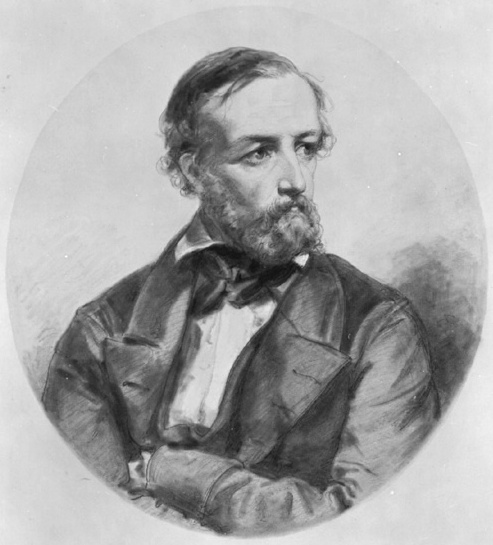
\includegraphics[height=2.9cm]{figures/mathematicians/Peter_Dirichlet.jpg} }}
    \qquad
    \subfloat[][\centering David Hilbert (1862--1943)]{{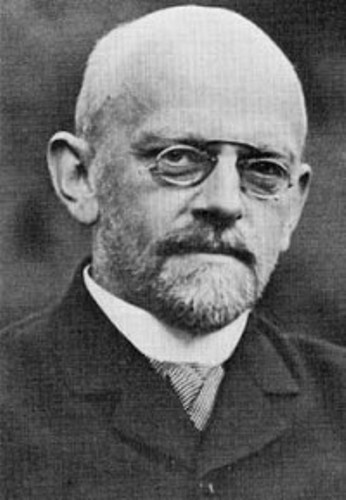
\includegraphics[height=2.9cm]{figures/mathematicians/David_Hilbert.jpeg} }}
    \qquad
    \subfloat[][\centering Walther Ritz (1878--1909)]{{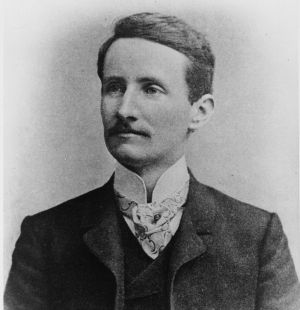
\includegraphics[height=2.9cm]{figures/mathematicians/Walther_Ritz.jpg} }}
    \qquad
    \subfloat[][\centering Boris Galerkin (1871--1945)]{{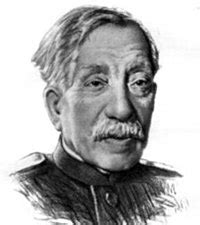
\includegraphics[height=2.9cm]{figures/mathematicians/Boris_Galerkin.jpeg} }}
    \qquad
    \subfloat[][\centering Sergei Sobolev (1908--1989)]{{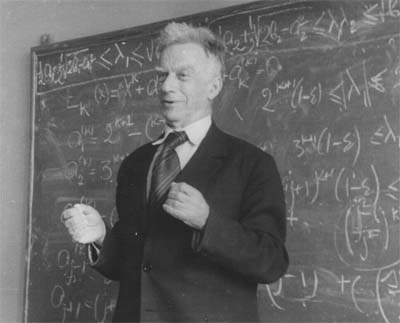
\includegraphics[height=3.4cm]{figures/mathematicians/Sergei_Sobolev.jpg} }}
    \qquad
    \subfloat[][\centering Laurent Schwartz (1915--2002)]{{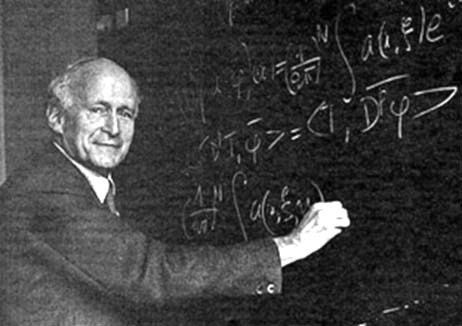
\includegraphics[height=3.4cm]{figures/mathematicians/Laurent_Schwartz.jpeg} }}
    \caption{Some key figures whose work precipitated modern developments in PDEs.}
    \label{fig:galerkin_mathematicians}
\end{figure}
In applications, the Navier-Stokes equations are primarily
solved on a computer, and a computer works with both finite data and finite precision. We will solve these equations by a \textit{Galerkin method}.
Galerkin methods
are particularly amenable to computer implementation, so much so that the whole process of geometric modelling, boundary condition handling,
residual minimisation, and solution reconstruction, can be automated (\cite{firedrake}, \cite{fenics_book}, \cite{DOLFIN}). We begin by
deriving two instances of Galerkin methods for Poisson's equation, performed on an irregular 2D domain to emphasize that the methods trivially extend
to complex geometries.
These methods are instances of a \textit{finite volume method} and a \textit{finite element method}.
Computer implementations are presented, which generate visualisations and quality metrics for the results.



\subsubsection{The Galerkin method}
The Galerkin method was established by engineer and mathematician Boris Galerkin (1871--1945) in a 1915 paper containing
an approximation method for the biharmonic equation of classical beam theory \cite{boris_galerkin}. Briefly, the principle of Galerkin is to
choose a space of approximations, today called ``test functions'', and solve for the test function which minimises a residual error with respect
to some function space norm. This norm is induced by a choice of what are now called the ``trial functions''. If the trial functions are the same as the test functions,
the residual is minimised with respect to the Euclidean norm.

As well as proving highly useful
in numerical applications, the methods of Galerkin (and preceding work by mathematicians such as Walther Ritz) proved important to further developments
in the mathematical theory of PDEs. A 1934 talk named ``Generalized Solutions to the Wave Equation'', by mathematician Sergei L. Sobolev (1908--1989),
precipitated the development
of generalised functions by Laurent Schwartz (1915-2002), integral to the modern study of PDEs
(\cite{sobolev_web_page}, \cite{one_hundred_years_galerkin}).
These developments are clarifications on the question: What do we mean when we speak of a solution to a PDE from physics? Galerkin's method
is much closer to the answer than, for example, the finite difference method.

\section{The equation to solve: Poisson's equation}

Among the fundamental PDEs
are the heat equation
    $$\Part{h}{t} = \Delta h + g$$
and Poisson's equation
\begin{equation}\label{poisson_compact}
    -\Delta h = g.
\end{equation}
The focus here is on the Dirichlet problem
\begin{equation}\label{poisson_dirichlet_problem}
    -\Delta h = g, \quad \left.h\right|_{\Gamma} = h_\Gamma,
\end{equation}
where $\Gamma$ is the boundary of the domain, and the domain is 2D.
Poisson's equation can be thought of as the steady-state version of the heat equation. The solution of a Poisson problem will be a crucial component
of the solution of the Stokes equations. It seems ideal to start by discussing
discretization methods for Poisson's equation \eqref{poisson_compact} in particular,
as it is likely the simplest non-trivial PDE. Poisson's equation \eqref{poisson_compact}, importantly,
is based on an integral conservation law.
An integral form will give clearer routes to discretizations which
have geometric meaning.
For example, the general integral conservation law \eqref{continuity_equation},
\begin{align*}
    \frac{d}{dt} \int_{\Omega_0} \phi\,dx = \int_{\Omega_0} s\,dx + \oint_{\pomn} \phi j \cdot \left(-\hat{n}\right)\,dx,
\end{align*}
is a geometric statement about fluxes
of quantity $\phi$ by $j$, quantified over arbitrary control volumes $\Omega_0$.
There are an infinite number of control volumes, and therefore an infinite number of equations which must hold, and there is an infinite dimensional
space of solutions to choose from. A key idea, then, is to choose a finite number of equations and a finite dimensional subspace of possible approximate solutions.
A supposed solution will be represented by the coefficients of some choice of basis functions for the subspace. Each equation will be checked exactly against this supposed solution.
To continue with this idea, we must write Poisson's equation \eqref{poisson_compact} in integral form.


\subsubsection{Deriving the heat and Poisson equation through diffusion processes}
The Poisson equation \eqref{poisson_compact} can be thought of as the steady state of some diffusion process with a source term $g$,
although this need not be its literal physical interpretation.
A diffusion process ``levels out'' some quantity, such as temperature or some chemical concentration.
A diffusion could intuitively be thought of as a
progressive ``blurring'',
such as in a camera defocus, and in fact many common image processing techniques use diffusion PDEs from physics \cite{tum}. We will stick with
the notion of ``temperature'' $h$ as the diffused quantity.
\textit{Fick's law of diffusion} is a constitutive relation giving the bulk flux of temperature $h$ as proportional to the negative gradient:
    $$hj = -\mu\nabla h,$$
where $\mu$ is called the diffusion coefficient.
This is one way of saying that the temperature tends to level out.
If we form a continuity equation \eqref{continuity_equation} for temperature, with source $s$, we get
\begin{equation}\label{heat_equation_integral}
    \frac{d}{dt} \int_{\Omega_0} h\,dx = \int_{\Omega_0} s\,dx + \oint_{\pomn} \mu \nabla h \cdot \hat{n}\,dx,
\end{equation}
which by application of Stokes' theorem becomes
\begin{equation}\label{heat_equation_differential}
    \frac{dh}{dt} = s + \nabla \cdot \left(\mu \nabla h\right).
\end{equation}
If we further assume that the diffusion coefficient $\mu$ is constant, we get
\begin{equation}\label{heat_equation_differential_constant}
    \frac{dh}{dt} = s + \mu\nabla \cdot \nabla h = s + \mu\Delta h,
\end{equation}
which is the standard heat equation.
The steady-state heat equation is then
\begin{equation}\label{poisson_equation}
    -\Delta h = g,
\end{equation}
where we let $g = s/\mu$ in the above.
This completes the derivation of Poisson's equation \eqref{poisson_compact}.
% which models steady-state diffusion processes and can be used to calculate gravitational or electrostatic potential fields.
In integral form, ``undoing'' the application of Stokes' theorem above, Poisson's equation is
\begin{equation}\label{poisson_equation_integral}
    \oint_{\pomn} -\nabla h\cdot \hat{n}\,dx = \int_{\omn} g\,dx \quad \text{for all control volumes $\Omega_0$.}
\end{equation}
Form \eqref{poisson_equation_integral} clearly shows that we are calculating a steady state,
as we are solving for $h$ such that the amount of heat that leaves $\Omega_0$ is the amount introduced into $\Omega_0$ by the source function.
The form \eqref{poisson_equation_integral}, rather than \eqref{poisson_compact}, will be the starting point for deriving Galerkin methods.

\subsubsection{So how do we discretize Poisson's equation?}
Thinking about the differential equation \eqref{poisson_differential_intro} leads to the \textit{finite difference method}, historically the first and
still very important in applications.

\begin{aside}
\textit{An aside: The finite difference method.}
\vskip 0.05in

\noindent
It is a theorem of Gauss that in Euclidean space $\mathbb{R}^3$ we have
\begin{equation}\label{gauss_euclidean_divergence}
    \nabla \cdot v = \Part{v_x}{x} + \Part{v_y}{y} + \Part{v_z}{z},
\end{equation}
and we get \eqref{poisson_compact} in the form
\begin{equation}\label{poisson_differential_intro}
    -\left(\frac{\partial^2 h}{\partial x^2}
           +\frac{\partial^2 h}{\partial y^2}
           +\frac{\partial^2 h}{\partial z^2}\right) = g.
\end{equation}
By forming secant approximations of the derivatives over a regular grid,
a linear system is formed, and the approximate solution is solved
for as a function of this grid.
However, it may be hard to give a real interpretation of what the solution samples at grid points say about the solution everywhere.
They could be coefficients of, for example, hat basis functions.
Yet a finite difference discretization of Poisson equation \eqref{poisson_compact} may not take this into account at all. One might feel that
limits have been taken too soon.
\end{aside}

We will not be using the finite difference method
\footnote{However, even if the spatial discretization is based on integral conservation laws, typically time-dependent problems
          are discretized with finite differences in the time dimension.}.
Starting with the integral form \eqref{poisson_equation_integral}, there are many routes to take to discretization.
Notice that there are two variables in \eqref{poisson_equation_integral}, although one is bound over universal quantification:
the function $h$ and the control volume $\Omega_0$.
The general Galerkin method very naturally appears when the ``space'' $\Omega_0$ resides in and the space $h$ resides in are reduced
such that the equations are both finite dimensional and well-determined.
Firstly, let's derive the conceptually simplest
discretization method of these spaces, the finite volume method.

% Consider a single conservation law as described in section \ref{conservation_laws}. This law
% was given in two forms, ``integral'' \eqref{continuity_equation}:
% \begin{equation*}
%     \frac{d}{dt} \int_{\Omega_0} \phi\,dx = \int_{\Omega_0} s\,dx + \int_{\pomn} \phi j \cdot \left(-\hat{n}\right)\,dx,
% \end{equation*}
% and ``differential'' \eqref{continuity_equation_differential}:
% \begin{equation*}
%     \Part{\phi}{t} = s - \nabla\cdot (\phi j).
% \end{equation*}

% \vskip 0.2in
% (figure)
% \vskip 0.2in
% 
% Finite element methods, and more generally Galerkin methods, live comfortably in the language of weak solutions, integral forms of partial differential equations,
% and the calculus of variations.
% To continue with this idea, we must write Poisson's equation \eqref{poisson_compact} in integral form.



\section{Discretizing Poisson's equation by finite volumes}\label{discretizing_poisson}
% ---NOTE: $H^1$ May be wrong.
% ---NOTE: Should discuss interpretation in terms of residual minimisation with respect to some norm.
% \vskip 0.5in
Equation \eqref{poisson_equation_integral} is quantified over an infinite number of control volumes $\Omega_0$.
These control volumes are in the interior of $\Omega$, as the solution at the boundary $\Gamma$ is specified by the Dirichlet boundary condition
$\left.h\right|_\Gamma = h_\Gamma$, and there is no flux information across $\Gamma$.
A simple idea is to choose a finite number of control volumes $\Omega_1,\cdots,\Omega_n$ (hence ``finite volumes''), and check that the flux integral holds over each of these.
We will then have $n$ equations on $h$. As this system will be underdetermined ($h$ has infinite degrees of freedom), we must
restrict $h$ to a finite dimensional space of approximations $\Phi^*$.

We begin by discussing the general construction of a finite volume method, but this will soon be made concrete with a simple, specific example of a 
finite volume discretization.


\subsection{The Dirichlet boundary condition and the test space}
The Dirichlet boundary condition $\left.h\right|_\Gamma = h_\Gamma$ specifies the boundary values for any solution.
However, the finite dimensional space $\Phi^*$ may not be able to exactly represent the boundary function $h_\Gamma$,
and therefore the first step is to approximate $h_\Gamma$ (for which there are many options, for example
projection in the $L^2$-norm or interpolation across a finite sampling of boundary points \cite{approximation_theory}). Choosing some $\phi_\Gamma \in \Phi^*$ with
    $$\left.\phi_\Gamma\right|_\Gamma \approx h_\Gamma,$$
we can define an ``interior'' function space
$$
    \Phi = \left\{h^* \in \Phi^* \mid \left.h\right|_\Gamma = 0 \right\},
$$
and the approximate solution $\tilde{h}$ will then be
$$
    \tilde{h} = \phi + \phi_\Gamma
$$
for some $\phi \in \Phi$.
In the finite volume and finite element literature the space $\Phi$ is called the test space.
Since we selected $n$ control volumes $\Omega_1,\cdots,\Omega_n$, the approximating space $\Phi^*$ must be chosen such that
$\Phi$ is $n$-dimensional. We can choose a basis for the test space,
    $$\Phi = \text{span}\left\{\phi_1,\cdots,\phi_n\right\}.$$
The problem is now to find a vector of coefficients of these test functions,
    $\hat{h} = (h_1, \cdots, h_n)^T,$
and reconstruct the solution as
    $$\tilde{h} = \phi + \phi_\Gamma,$$
where $\phi$ is the ``interior variation''
    $$\phi = \Phi\cdot \hat{h} \coloneqq h_1\phi_1 + \cdots + h_n\phi_n.$$

\subsection{Forming a linear system}
The integral-conservation-law form \eqref{poisson_equation_integral} of Poisson's equation \eqref{poisson_compact}
now directly indicates a method of approximation. Letting $h$ be approximated by $\tilde{h} = \phi + \phi_\Gamma$ (where $\phi \in \Phi$ is unknown and $\phi_\Gamma \in \Phi^*$ is known),
and restricting the flux integrals to the control volumes $\Omega_1,\cdots,\Omega_n$, the conservation law \eqref{poisson_equation_integral} becomes
\begin{equation}\label{poisson_equation_integral_fvm}
    \oint_{\partial\Omega_j} -\nabla \left(\phi + \phi_\Gamma\right) \cdot \hat{n}\,dx = \int_{\Omega_j} g\,dx \quad\quad j=1,\cdots,n.
\end{equation}
The ``interior variation'' $\phi = \Phi\cdot \hat{h}$ is the only unknown, so we can move all knowns to the right-hand side
and expand $\phi$ in terms of the basis test functions $\phi_1,\cdots,\phi_n$:
\begin{equation}\label{poisson_equation_integral_fvm_knowns_unknowns}
    \oint_{\partial\Omega_j} -\nabla \left(\sum_{i=1}^nh_i\phi_i\right) \cdot \hat{n}\,dx =
            \int_{\Omega_j} g\,dx
            + \oint_{\partial\Omega_j} \nabla \phi_\Gamma \cdot \hat{n}\,dx
 \quad\quad j=1,\cdots,n.
\end{equation}
By linearity, to emphasize the separate integrals that need to be computed, the above equation can be written as
\begin{equation}\label{poisson_equation_integral_discretized}
    \sum_{i=1}^n h_i\oint_{\pom_j} -\nabla \phi_i \cdot \hat{n}\,dx =
            \int_{\Omega_j} g\,dx
            + \oint_{\partial\Omega_j} \nabla \phi_\Gamma \cdot \hat{n}\,dx
 \quad\quad j=1,\cdots,n.
\end{equation}
It is seen here that there must be some restrictions on the $\phi_i$ and $\phi_\Gamma$.
Formally, they must be in the Sobolev space $H^1(\Omega)$
(--- NOTE: This is probably wrong, as the integrals are over internal cell boundaries and the boundary $\Gamma$. Need to read
about $H^{\text{div}}$)
This simply means that they must have a gradient defined ``almost everywhere''.
It does not matter if the gradient is not defined at isolated lower-dimensional subsets, as these make no contribution to
the integral. The system \eqref{poisson_equation_integral_discretized} can be written in matrix form as
\newcommand{\integralentry}[2]{\oint_{\pom_{#1}}-\nabla\phi_{#2}\cdot\hat{n}\,dx}
\newcommand{\integralrhsentry}[1]{\int_{\om_{#1}}g\,dx + \oint_{\pom_{#1}}\nabla\phi_\Gamma\cdot\hat{n}\,dx}
\begin{equation}\label{poisson_matrix_equation}
\begin{split}
    A\hat{h}
    &= \begin{bmatrix}
            \integralentry{1}{1} & \cdots & \integralentry{1}{n} \\
            \vdots & & \vdots \\
            \integralentry{n}{1} & \cdots & \integralentry{n}{n}
    \end{bmatrix}
    \begin{bmatrix} h_1 \\ \vdots \\ h_n \end{bmatrix}
    \\
    &= \begin{bmatrix} \integralrhsentry{1} \\ \vdots \\ \integralrhsentry{n}  \end{bmatrix}
    = \hat{f}.
\end{split}
\end{equation}
This system is solved for the coefficients of combination $\hat{h} = (h_1 \cdots h_n)^T$, and the approximate
solution is constructed as $\tilde{h} = \Phi\cdot\hat{h} + \phi_\Gamma$.
If the control volumes $\Omega_1,\cdots,\Omega_n$ and test space $\Phi = \text{span}\left\{\phi_1,\cdots,\phi_n\right\}$
are chosen well, this linear system will be nonsingular and hopefully well-conditioned.
If the chosen control volumes join together in the interior of $\Omega$ like pieces of a puzzle, this gives a conservative system of balanced fluxes, but it is another question whether the approximation
$\tilde{h}$ is good.

\subsection{A piecewise linear finite volume triangulation scheme}
Possibly the simplest scheme is to triangulate $\Omega$ as
    $\bigcup_i T_i,$
such that there are $n$ interior vertices $p_1,\cdots,p_n$, and $n_\Gamma$ boundary vertices $p^\Gamma_1,\cdots,p^\Gamma_{n_\Gamma}$, and $n_T$ triangles
$T_1,\cdots,T_{n_T}$. An example triangulation of an ellipse-shaped domain is shown in figure \ref{triangulation}.
\begin{figure}[H]
    \begin{center}
        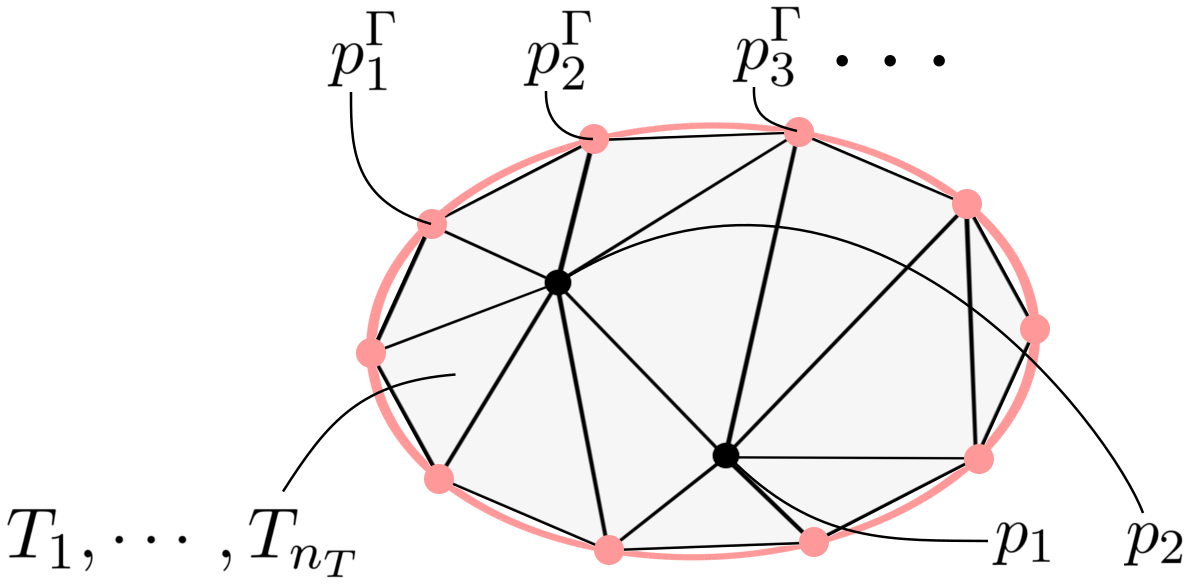
\includegraphics[width=0.53\linewidth]{figures/triangulation/triangulation.png}
    \end{center}
    \caption{\scriptsize
        The domain $\Omega$ is partitioned into $n_T = 12$ triangular cells $T_1\cdots T_{12}$. The boundary is sampled at $n_\Gamma = 10$ points
        $p^\Gamma_1,\cdots,p^\Gamma_{10}$.
        There are $n = 2$ interior points, $p_1$ and $p_2$.
    }
    \label{triangulation}
\end{figure}

\subsubsection{The test space}
Firstly, there is a clear choice of function space $\Phi^*$, which satisfies the $H^1$ condition
(NOTE: Is $H^1$ necessary? Need to check conditions for finite volumes), consisting of piecewise linear ``hat'' basis functions
at each interior or boundary vertex,
\newcommand{\hatfun}[1]{\text{Hat}(#1)}
$$
    \Phi^* = \text{span}\left\{
        \hatfun{p_1},\cdots,\hatfun{p_n},
        \hatfun{p^\Gamma_1},\cdots,\hatfun{p^\Gamma_{n_\Gamma}}
    \right\}.
$$
The hat function at a vertex has value $1$ at that vertex and value $0$ at its neighbours.
The test space (which is zero on the boundary $\Gamma$) is then
\begin{align*}
    \Phi &= \text{span}\left\{
        \hatfun{p_1},\cdots,\hatfun{p_n}
    \right\} = \text{span}\left\{\phi_1,\cdots,\phi_n\right\},
\end{align*}
where $\phi_i \coloneqq \text{Hat}(p_i)$.
One of these basis functions for the ellipse-shaped domain is shown in figure \ref{ellipse_partition}.
\begin{figure}[H]
    \begin{center}
        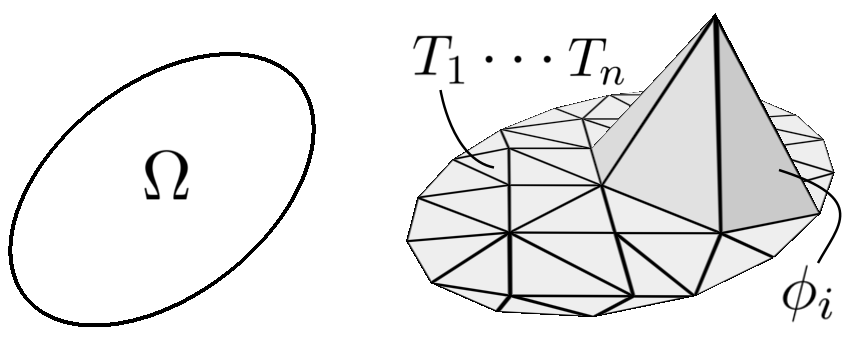
\includegraphics[width=0.53\linewidth]{figures/hat.png}
    \end{center}
    \caption{\scriptsize
        The domain $\Omega$ is partitioned into triangular cells $T_1\cdots T_{n_T}$. One example of a hat basis function $\phi_i$ is shown, where
        the vertical axis is the basis function value.
    }
    \label{ellipse_partition}
\end{figure}

\newpage
\subsubsection{Approximating the boundary values}
One simple approximation of $\left.h\right|_\Gamma = h_\Gamma$ is
\begin{equation}\label{boundary_approximation}
    \phi_\Gamma = h_\Gamma(p^\Gamma_1)\hatfun{p^\Gamma_1}
                + \cdots
                + h_\Gamma(p^\Gamma_{n_\Gamma})\hatfun{p^\Gamma_{n_\Gamma}},
\end{equation}
which is a piecewise linear interpolation when restricted to the boundary $\Gamma$. The approximation $\phi_\Gamma$ for some boundary
function $h_\Gamma$ is shown in figure \ref{boundary}.
\begin{figure}[H]
    \begin{center}
        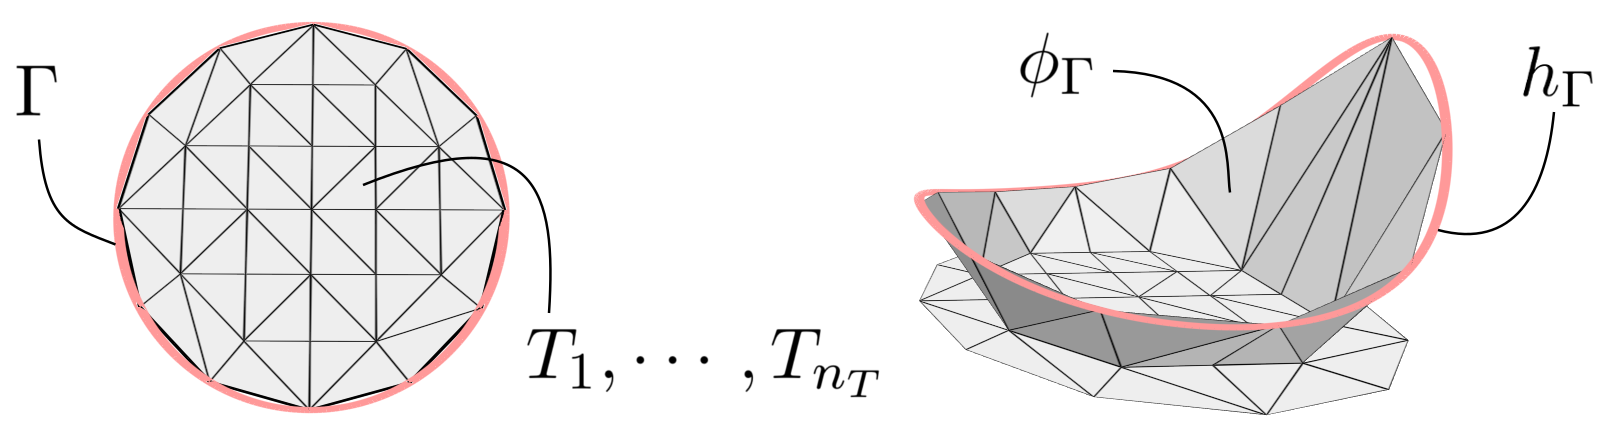
\includegraphics[width=0.9\linewidth]{figures/boundary/boundary.png}
    \end{center}
    \caption{\scriptsize
        A circle domain $\Omega$ with boundary $\Gamma$ is tessellated by triangles $T_1,\cdots,T_{n_T}$.
        The boundary function $h_\Gamma$ is approximated by $\phi_\Gamma$, a linear combination of hat functions centred at the boundary vertices.
    }
    \label{boundary}
\end{figure}
This approximation $\phi_\Gamma$ is added to the ``interior variation'' $\phi = \Phi\cdot\hat{h}$ to construct a possible solution.
When a linear solver is given the linear system \eqref{poisson_matrix_equation}, it will find the interior variation $\phi$
which minimises some residual norm. An iterative solver, for example, can then be thought of as progressively varying a thin membrane attached
to the boundary curve,
until the residual error is sufficiently small. This construction is shown in figure \ref{laplaceboundary}.
\begin{figure}[H]
    \begin{center}
        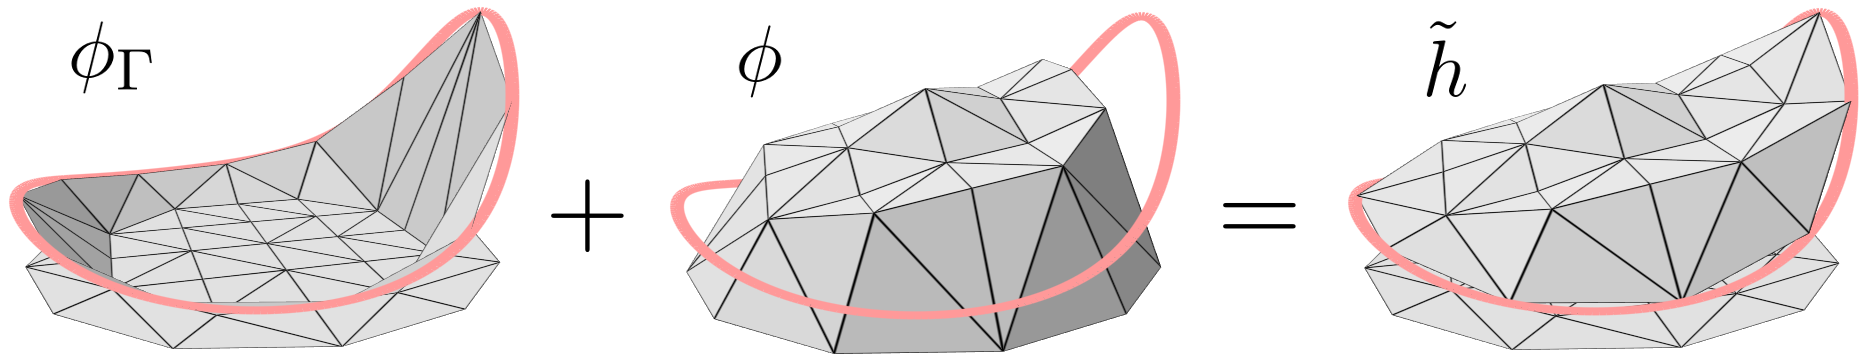
\includegraphics[width=1\linewidth]{figures/laplaceboundary/laplaceboundaryv2.png}
    \end{center}
    \caption{\scriptsize
        The fixed boundary approximation $\phi_\Gamma$ is added to a variable interior variation $\phi$ to give a possible approximate solution $\tilde{h}$.
        This possible solution can be checked by integration against the trial control volumes $\Omega_1,\cdots,\Omega_n$.
    }
    \label{laplaceboundary}
\end{figure}
\subsubsection{Choosing a finite number of control volumes}
If we choose some characteristic ``triangle centre'' for each triangle, then we can associate to the interior vertices
$p_1,\cdots,p_n$ a set of domains $\Omega_1,\cdots,\Omega_n$. Each $\Omega_i$ is determined by the polygon which joins the centres of the triangles
incident to $p_i$.
Two common choices for the triangle centre are the barycentre, which is the average position of the three vertices, and the circumcentre,
which is the centre of the unique circle passing through the three vertices. The circumcentre scheme gives what are called
``Voronoi cells'' due to their relation to Voronoi diagrams in computational geometry \cite{orourke}.
The resulting cell decompositions are displayed in figure
\ref{cell_decompositions}.

\begin{figure}[H]
    \begin{center}
        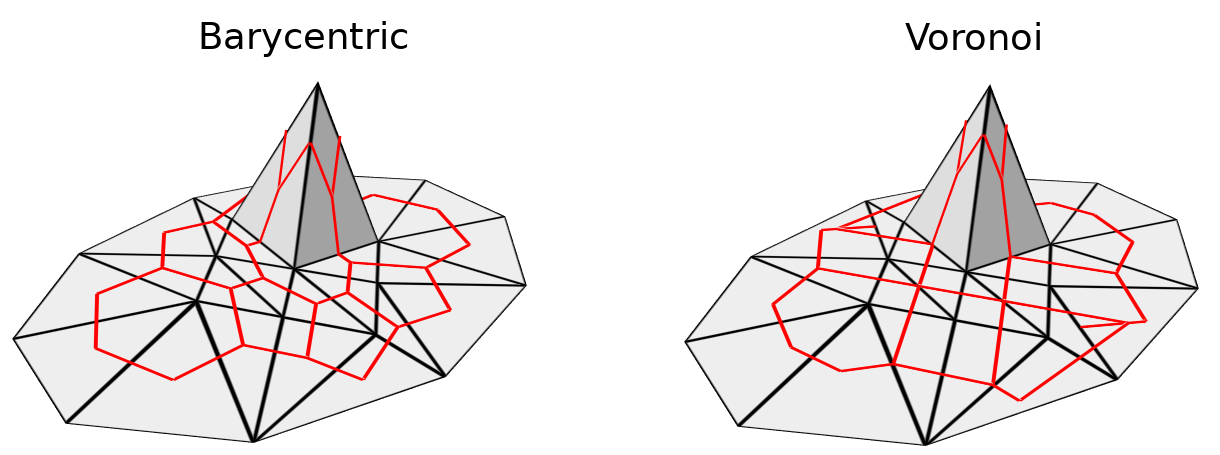
\includegraphics[width=0.7\linewidth]{figures/cell.png}
    \end{center}
    \caption{\scriptsize
        The domain $\Omega$ is partitioned into triangular cells $T_1\cdots T_{n_T}$.
        Flux integrals are taken over $n$ polygonal cells, one for each internal vertex $p_i$, for example using triangle barycentres or circumcentres.
    }
    \label{cell_decompositions}
\end{figure}
Notice that, in the circumcentre case, the thin triangles do not contain their circumcentre, and therefore each cell boundary is not necessarily
contained in a single fan of triangles. Notice also that the Voronoi polygon passes through the midpoints of each edge incident to $p_i$.
This midpoint property will soon prove useful in computing integrals, but the resulting exposition will be clearer if we can also
assume that the cell boundary \textit{is} contained in a single fan of triangles. Therefore we define the \textit{mixed Voronoi cell} \cite{polygon_mesh_processing},
where a wayward circumcentre is pulled back to the opposite edge.

\vskip 0.2in
(draw this)
\vskip 0.2in

The scheme as described so far, consisting of a triangle mesh, hat test functions, and barycentric, Voronoi, or mixed Voronoi control volumes,
has found some success, especially in the domain of geometry processing (\cite{polygon_mesh_processing}, \cite{ddg_triangulated}).
We will work with the mixed Voronoi cells.

\subsection{Computing the linear system by closed form integration}\label{fvm_closed_form}
Now that we have chosen a specific finite volume discretization, given a domain triangulation we can compute
the coefficients of the linear system \eqref{poisson_matrix_equation} and solve for $\hat{h}$, giving
the approximate solution $\tilde{h} = \phi_\Gamma + \Phi\cdot \hat{h}$.
By fortuitous circumstances, these integrals actually have simple closed forms.
(This is with the exception of the heat source integrals $\int_{\Omega_j}g\,dx$,
which may require numerical integration if the heat source $g$ is not restricted to $\Phi^*$.)

It will be more convenient to start again with the trial flux integral
\newcommand{\fvmintegral}{
\oint_{\pom_j} -\nabla \tilde{h}\cdot\hat{n}\,dx
}
\begin{equation}\label{fvm_integral}
\fvmintegral,
\end{equation}
rather than with the expanded linear system \eqref{poisson_matrix_equation}.
By linearity, the $\nabla$ in $\nabla\tilde{h}$ ``falls through'' the expansion of $\tilde{h}$:
% $\nabla \tilde{h}$ is a combination of gradients of basis functions of $\Phi^*$:
\begin{equation}\label{gradient_expansion}
    \nabla \tilde{h} = \nabla\phi_\Gamma + \nabla\phi
             = \sum_{i=1}^{n_\Gamma}h_\Gamma(p^\Gamma_i)\nabla\phi^\Gamma_i + \sum_{i=1}^n h_i\nabla\phi_i.
\end{equation}
By linearity the integral \eqref{fvm_integral} becomes
\begin{equation}\label{fvm_integral_linearity_expanded}
    \sum_{i=1}^{n_\Gamma}\left[h_\Gamma(p^\Gamma_i)\oint_{\pom_j}-\nabla\phi^\Gamma_i\cdot\hat{n}\,dx\right]
    + \sum_{i=1}^n\left[h_i\oint_{\pom_j}-\nabla\phi_i\cdot\hat{n}\,dx\right].
\end{equation}

% We therefore need only compute the integrals
% $$
%     \int_{\Omega_j} \nabla\phi_i \cdot \hat{n}\,dx.
% $$
Now consider a certain flux integral \eqref{fvm_integral} over control volume $\Omega_j$. We will reexpress the above integral
in ``local'' terms.
%local terms------------------------------------------------------------
\newcommand{\definelocalterms}[1]{
\begin{aside}
\textit{Some local indexing definitions.}\\
\vskip -0.1in
Let $v = p_j$ be the interior vertex corresponding to #1, and denote by $v_1, \cdots, v_k$ its adjacent vertices (either in the interior
or on the boundary), and by $T^v_1 \cdots T^v_k$ its adjacent triangles. Triangle $T^v_l$ joins $v,v_l,v_{l+1}$ where addition wraps around from $k$ to $1$.
As it will be necessary to relate these local indices (denoted $l$) to the global vertex indices (denoted $i$), define an index map by
    $$I(l) = \text{the global index $i$ of the $p_i$ corresponding to adjacent vertex $v_l$},$$
which is valid only when $v_l$ is an interior vertex.
\end{aside}
}
\definelocalterms{the control volume $\Omega_j$}
%end local terms------------------------------------------------------------
The vertex $v$ corresponds to a single trial flux integral over the surrounding Voronoi cell $\Omega_j$.
As the hat functions have compact support, $\Omega_j$ only intersects the domains of the hat function $\phi_j$ and those corresponding
to the adjacent vertices. Name these basis functions $\phi_j = \phi_v$ and $\phi_{v_1}, \cdots \phi_{v_k}$.
Then the local form of the flux integral \eqref{fvm_integral} is
\begin{equation}\label{fvm_integral_vertex}
    \fvmintegral = h_j\oint_{\pom_j}-\nabla\phi_v\cdot\hat{n}\,dx + \sum_{l=1}^{k}h_{v_l}\oint_{\pom_j}-\nabla\phi^v_l\cdot\hat{n}\,dx,
\end{equation}
where $h_{v_i}$ is defined as
\newcommand{\hvidefinition}{
\begin{align*}
    h_{v_i} =
    \left\{\begin{array}{lr}
        h_\Gamma(p^\Gamma_i) &\text{if $v_i$ is a boundary vertex,}\\
        h_{I(v_i)} &\text{if $v_i$ is an interior vertex}.\\
        \end{array}\right.
\end{align*}
}
\hvidefinition
The $\phi_v$ and $\phi_{v_1},\cdots,\phi_{v_k}$ are hat functions which are linear when restricted to each triangle
$T^v_1,\cdots,T^v_k$. Therefore the gradients $\nabla\phi_v$ and $\nabla\phi_{v_1},\cdots,\nabla\phi_{v_k}$ are constant
on those triangles. We can break the closed flux integrals in \eqref{fvm_integral_vertex} into flux integrals restricted to each triangle adjacent to $v$, giving
\begin{equation}\label{fvm_integral_vertex_triangles}
    \fvmintegral = \sum_{t=1}^k\left[\int_{\Omega_j \cap T^v_t}-\nabla\phi_v\cdot\hat{n}\,dx + \sum_{l=1}^{k}h_{v_l}\int_{\Omega_j \cap T^v_t}-\nabla\phi^v_l\cdot\hat{n}\,dx\right].
\end{equation}
We can simplify matters by focusing on just one adjacent triangle $T^v_t = T$, between vertices
$v,v_t,v_{t+1}$. This triangle $T$ only overlaps with the domains of the hat functions centred at $v,v_t,v_{t+1}$, so we
now only need to compute
$$
\int_{\Omega_j \cap T} -\nabla\phi_v\cdot\hat{n}\,dx \text{\quad and \quad} 
\int_{\Omega_j \cap T} -\nabla\phi_{v_t}\cdot\hat{n}\,dx \text{\quad and \quad} 
\int_{\Omega_j \cap T} -\nabla\phi_{v_{t+1}}\cdot\hat{n}\,dx.
$$
This is simple because the gradients are constant on $\Omega_j \cap T_t^v$.

\vskip 0.2in
(figure)
\vskip 0.2in

The Voronoi polygon joins the midpoints $m^\pr = \frac{1}{2}(v + v_t)$ and $m^\ppr = \frac{1}{2}(v + v_{t+1})$, taking a detour to a point within $T$.

\vskip 0.2in
(figure)
\vskip 0.2in

However, since the gradient vector fields are constant, they are conservative, and we can simplify the domain $\Omega_j \cap T$ to the line segment $L$ between
the midpoints $m^\pr$ and $m^\ppr$. Since the gradients are constant on $T$, these integrals are the length of $L$ multiplied by one ``sample'' flux across $L$.
This can be done easily, by noticing $L$ is parallel with and half the length of the line segment between $v_t$ and $v_{t+1}$.
We can then compute the integrals as:
\begin{equation}\label{fvm_integrals_closed}
    \frac{1}{2}\nabla\phi_v\cdot(v_{t+1} - v_t)^\perp,\text{\quad and \quad}
    \frac{1}{2}\nabla\phi_{v_t}\cdot(v_{t+1} - v_t)^\perp,\text{\quad and \quad}
    \frac{1}{2}\nabla\phi_{v_{t+1}}\cdot(v_{t+1} - v_t)^\perp,
\end{equation}
where $(v_{t+1} - v_t)^\perp$ is the vector $v_{t+1} - v_t$ rotated $90$ degrees anticlockwise.
We now only need the constant gradients on $T$. This requires some simple geometry. As this construction is the same for each vertex, consider an anticlockwise ordering of $v,v_t,v_{t+1}$, named $v^\pr,v^\ppr,v^\pppr$.

\vskip 0.2in
(figure of a rectangle drawn around the triangle, and the perpendicular direction, with width and height labels)
\vskip 0.2in

We must normalize this vector and then divide by the height of this rectangle, as the slope is inversely proportional to the rectangle height.
This gives the gradient
$$
    \nabla\phi_{v^\pr} = \left.\frac{(v^\pppr - v^\ppr)^\perp}{\norm{v^\pppr - v^\ppr}}\right/h = \frac{(v^\pppr - v^\ppr)^\perp}{wh}.
$$
Finally, $\text{Area}(T) = wh/2$, so we can write the gradients as
\begin{equation}\label{fvm_gradients}
    \nabla\phi_v = \frac{\left(v_{t+1} - v_t\right)^\perp}{2\text{Area}(T)},\text{\quad and \quad}
    \nabla\phi_{v_t} = \frac{\left(v - v_{t+1}\right)^\perp}{2\text{Area}(T)},\text{\quad and \quad}
    \nabla\phi_{v_{t+1}} = \frac{\left(v_t - v\right)^\perp}{2\text{Area}(T)}.
\end{equation}

Plugging the gradients \eqref{fvm_gradients} into the closed form integrals \eqref{fvm_integrals_closed}, we get
\begin{equation}\label{fvm_closed_form_integrals}
\begin{split}
    \int_L -\nabla\phi_v\cdot\hat{n}\,dx
        &= \frac{1}{4\text{Area}(T)}\norm{v_{t+1} - v_t}^2,\\
    \int_L -\nabla\phi_{v_t}\cdot\hat{n}\,dx
        &= \frac{1}{4\text{Area}(T)}(v - v_{t+1})\cdot(v_{t+1} - v_t),\\
    \int_L -\nabla\phi_{v_{t+1}}\cdot\hat{n}\,dx
        &= \frac{1}{4\text{Area}(T)}(v_t - v)\cdot(v_{t+1} - v_t),
\end{split}
\end{equation}
where the 90-degree rotation has been removed, as it preserves the dot product.
With these closed forms, we can express the original integral as
\begin{equation}\label{flux_integral_summation}
\begin{split}
&\oint_{\pom_j} -\nabla \tilde{h}\cdot\hat{n}\,dx\\
    &=
    \sum_{t=1}^k
        \frac{1}{4\text{Area}(T^v_t)}
        \left[
        h_j \norm{v_{t+1} - v_{t}}^2
        +h_{v_t}(v - v_{t+1})\cdot(v_{t+1} - v_{t})
        +h_{v_{t+1}}(v_t - v)\cdot(v_{t+1} - v_{t})
        \right].
\end{split}
\end{equation}
This directly indicates an effective algorithm for constructing the linear system.

\subsubsection{Integrating the source function}
One more thing is needed, however. The right-hand side vector of \eqref{poisson_matrix_equation} contains source integrals
    $$\int_{\om_j}g\,dx,$$
so we require some numerical integration.
The simplest choice is a ``rectangle rule'', where we sample the source function $g$ at the interior vertex
$p_j$, then assume that $g$ is constant over $\om_j$. This gives the approximation
\begin{equation}\label{fvm_source_approximation}
    \int_{\om_j}g\,dx \approx g(p_j)\text{Area}(\om_j).
\end{equation}
The computation of the mixed Voronoi cell area $\text{Area}(\om_j)$ can be achieved with some routine geometric calculations.
Iterating over each triangle incident to $p_j$, compute the cell segment area as the area of two triangles, the second triangle depending on whether
the computed circumcentre lies inside or outside the triangle.

\vskip 0.2in
(draw this)
\vskip 0.2in

\subsection{The resulting matrix assembly algorithm}
Using the expression \eqref{flux_integral_summation}, the linear system
\eqref{poisson_matrix_equation} can be constructed by iterating over each interior vertex $v$, then each adjacent triangle,
and computing these closed form integrals.
Each adjacent triangle corresponds to two vertices incident to $v$, and for each of these vertices,
either a value is placed in either the system matrix or the right-hand side is adjusted,
depending on whether the triangle vertex is in the interior or on the boundary. Also, while iterating over the interior vertices,
the corresponding source integral is approximated by \eqref{fvm_source_approximation}, and the result is added to the right-hand side vector.
Pseudocode for this algorithm is given below.


% Routine name
\newcommand{\poissonfvmmatrixassembly}{Poisson\_FVM\_Matrix\_Assembly}

\newcommand{\totaltrianglearea}{\text{total\_triangle\_area}}
\begin{algorithm}\label{alg:assembly}

% https://tex.stackexchange.com/questions/64204/mutliple-inputs-with-line-breaking
\newlength\mylen
\newcommand\mydata[1]{%
  \settowidth\mylen{\KwData{}}%
  \setlength\hangindent{\mylen}%
  \hspace*{\mylen}#1\\}

\SetKwProg{Fn}{Routine}{\string:}{}
\SetKwProg{Def}{Define function}{\string:}{}
\Fn{\poissonfvmmatrixassembly}{
    \SetAlgoLined
    \KwData{Domain $\Omega$ with boundary $\Gamma$.}
    \mydata{Heat source function $g : \Omega\rightarrow \mathbb{R}$.}
    \mydata{Dirichlet boundary function $h_\Gamma : \Gamma \rightarrow \mathbb{R}$.}
    \mydata{Triangulation of $\Omega$ consisting of:}
    \mydata{\qquad Interior vertices $p_1,\cdots,p_n$.}
    \mydata{\qquad Boundary vertices $p^\Gamma_1,\cdots,p^\Gamma_{n_\Gamma}$.}
    \mydata{\qquad Triangles $T_1,\cdots,T_{n_T}$.}
    \KwResult{
        % Approximate solution $\tilde{h}:\Omega\rightarrow\mathbb{R}$ of the boundary value problem \eqref{poisson_dirichlet_problem},\\
        % \qquad\qquad\qquad\qquad $-\Delta h = g$, $\left.h\right|_\Gamma = h_\Gamma$.
        The coefficients $(A, \hat{f})$ of the system $A\hat{h} = \hat{f}$ \eqref{poisson_matrix_equation},
        which can be solved by the caller for $\hat{h}$ in order to reconstruct
        an approximate solution $\tilde{h}:\Omega\rightarrow\mathbb{R}$ of the boundary value problem \eqref{poisson_dirichlet_problem},\\
        \qquad\qquad\qquad\qquad $-\Delta h = g$, $\left.h\right|_\Gamma = h_\Gamma$.
    }
    $A \leftarrow \text{$n\times n$ zero matrix}$\;
    $\hat{f} \leftarrow \text{length $n$ zero vector}$\;
    \For{$j = 1,\cdots,n$}{
        Let $v$ denote the interior vertex $p_j$.\\
        Let $v_1,\cdots,v_k$ denote the vertices adjacent to $v$.\\
        Let $T^v_1,\cdots,T^v_k$ denote the triangles adjacent to $v$.\\
        (Triangle $T_t$ joins vertices $v,v_t,v_{t+1}$.)\\
        \For{$t = 1,\cdots, k$}{
            $C \leftarrow \frac{1}{4\text{Area}(T)}$\;
            $A[j,j] \leftarrow A[j,j] + C\norm{v_{t+1} - v_t}^2$\;
            \uIf{$v_t$ is on the boundary}{
                $\hat{f}[I(t)] \leftarrow \hat{f}[I(t)] - h_\Gamma(v_t)C(v - v_{t+1})\cdot(v_{t+1}-v_t)$\;
            }
            \Else{
                $A[j, I(t)] \leftarrow A[j, I(t)] + C(v - v_{t+1})\cdot(v_{t+1} - v_t)$\;
            }
            \uIf{$v_{t+1}$ is on the boundary}{
                $\hat{f}[I(t+1)] \leftarrow \hat{f}[I(t+1)] - h_\Gamma(v_{t+1})C(v_t - v)\cdot(v_{t+1}-v_t)$\;
            }
            \Else{
                $A[j, I(t+1)] \leftarrow A[j, I(t+1)] + C(v_t - v)\cdot(v_{t+1} - v_t)$\;
            }
        }
        $\hat{f}[j] \leftarrow \hat{f}[j] + \text{Control\_Volume\_Area}(\Omega_j)\cdot g(v)$\;
    }
    \Return{$(A, \hat{f})$}\;
    % Solve $A\hat{h} = b$ for $\hat{h} = (h_1,\cdots,h_n)^T$\;
    % $\tilde{h} \leftarrow \sum_{j=1}^n h_j\text{Hat}(p_j) + \sum_{j=1}^{n_\Gamma} h_\Gamma(p_j^\Gamma)\text{Hat}(p_j^\Gamma)$\;
    % \Return{$\tilde{h}$}\;
}
    % \caption{Pseudocode for the described finite volume method for the Poisson boundary value problem \eqref{poisson_dirichlet_problem}.}
    \caption{Pseudocode for the described finite volume matrix assembly process for the Poisson boundary value problem \eqref{poisson_dirichlet_problem}.}
\end{algorithm}
\newpage

\subsection{The resulting finite volume algorithm}
We now have an effective algorithm for approximating Poisson's equation:
\begin{enumerate}
    \item Partition the 2D domain $\Omega$ into triangles $T_1,\cdots,T_{n_T}$. This determines the hat basis functions $\phi_1,\cdots,\phi_n$
         and the mixed Voronoi cells $\Omega_1,\cdots,\Omega_n$.
    \item Form the matrix and right-hand side in \eqref{poisson_matrix_equation} with the algorithm \ref{alg:assembly}.
    \item Solve the resulting linear system for $\hat{h}$, and construct the solution as $\tilde{h} = \phi_\Gamma + \Phi\cdot\hat{h}$.
\end{enumerate}
Each of these steps is conceptually well-separated into the domains of
mesh generation, matrix assembly, and numerical linear algebra. The above pseudocode \ref{alg:assembly} is a matrix assembly algorithm.
It assumes that there is already a domain triangulation, and constructs the linear system \eqref{poisson_matrix_equation}.
Although we have addressed the
problem of matrix assembly, specific to this particular finite volume method, mesh generation and numerical linear algebra can be delegated to external libraries.
The full solve algorithm is given below.

\begin{algorithm}\label{alg:fvm}

\newcommand\mydata[1]{%
  \settowidth\mylen{\KwData{}}%
  \setlength\hangindent{\mylen}%
  \hspace*{\mylen}#1\\}

\SetKwProg{Fn}{Routine}{\string:}{}
\SetKwProg{Def}{Define function}{\string:}{}
\Fn{Solve\_Poisson\_FVM}{

    \SetAlgoLined
    \KwData{Domain $\Omega$ with boundary $\Gamma$.}
    \mydata{Heat source function $g : \Omega\rightarrow \mathbb{R}$.}
    \mydata{Dirichlet boundary function $h_\Gamma : \Gamma \rightarrow \mathbb{R}$.}
    \KwResult{
        Approximate solution $\tilde{h}:\Omega\rightarrow\mathbb{R}$ of the boundary value problem \eqref{poisson_dirichlet_problem},\\
        \qquad\qquad\qquad\qquad $-\Delta h = g$, $\left.h\right|_\Gamma = h_\Gamma$.
    }
    \emph{// Mesh generation}\\
    $\text{triangulation} \leftarrow \text{Generate\_Triangulation}(\Omega)$\;
    \emph{// Matrix assembly}\\
    $(A,\hat{f}) \leftarrow \text{\poissonfvmmatrixassembly}(\Omega, g, h_\Gamma, \text{triangulation})$\;
    \emph{// Linear solve}\\
    Solve $A\hat{h} = \hat{f}$ for $\hat{h}$.\\
    \emph{// Solution reconstruction}\\
    $\tilde{h} \leftarrow \sum_{j=1}^n h_j\text{Hat}(p_j) + \sum_{j=1}^{n_\Gamma} h_\Gamma(p_j^\Gamma)\text{Hat}(p_j^\Gamma)$\;
    \Return{$\tilde{h}$}\;
}
\end{algorithm}

The routine \textbf{Generate\_Triangulation} is provided by a mesh generator, and 
the $\textbf{Solve}$ routine is provided by a numerical linear algebra library.
\subsubsection{Mesh generation}
Mesh generation is a huge field. However, there are only two essentials for the handling of 2D domains and piecewise linear triangulations
--- a mesh data structure and a triangulator. Typically a mesh data structure will be provided by a separate library,
and the data organization (e.g., vertex, triangle, and adjacency information) will be designed to facilitate the kinds
of mesh traversals performed during matrix assembly. This is typically some variant of a ``halfedge'' data structure \cite{polygon_mesh_processing},
implemented in libraries such as Geometry Central \cite{geometry_central},
the Polygon Mesh Processing library \cite{polygon_mesh_processing_library}, and OpenMesh \cite{openmesh}.

A mesh data structure is a foundational component of mesh generation systems. For 2D domains, a somewhat regular sampling of points on the boundary
and interior, followed by triangulation of these points, can suffice for a piecewise-linear finite volume mesh.
The Triangle \cite{triangle} library, for example, contains a single very efficient and robust C routine (consisting of 16k lines of highly optimized code)
for performing Delaunay triangulations \cite{orourke}
on 2D domains,
with the specific goal of creating robust finite element meshes.

\subsubsection{Numerical linear algebra}
The solution of large linear systems is a vast topic. PDE solvers are typically clients
of standard, robust linear and non-linear solver libraries, such as Argonne National Laboratory's PETSc libraries \cite{petsc}
and the smaller-scale C\texttt{++} libraries Armadillo \cite{armadillo} and Eigen \cite{eigen}.
A PDE solver will typically pass either a full matrix to the linear solver (dense or sparse),
or provide the linear solver with callback routines that give it access to the system coefficients when they are needed.

--- Discuss sparsity here.

\subsection{An implementation in C\texttt{++}}
I have implemented algorithm \ref{alg:fvm} in C\texttt{++}.
This code uses a simple mesh generator based on the C library Triangle \cite{triangle}. Triangle is given a list of points
and boundary points, and generates a Delaunay triangulation \cite{orourke}. This triangulation is then converted to a halfedge mesh data structure
based on the ideas in the Geometry Central library \cite{geometry_central}.
The matrix is constructed as a flat array of indices and coefficients, which are then converted to CRS (compressed row storage) form.
The system is solved with a sparse LU factorisation method provided by the C\texttt{++} Eigen library \cite{eigen}.
With these interfaces, the resulting C\texttt{++} was almost a direct transliteration of the pseudocodes \ref{alg:fvm} and \ref{alg:assembly}.

The implemented matrix assembly algorithm has linear space and time complexity in the number of mesh vertices,
and all data is generated and accessed in flat buffers, giving good cache performance.
The only superlinear stage is the system solve, which is handled by Eigen \cite{eigen}.
All computations have been performed with double precision floating point.


\subsection{Validating the method}
In order to validate this algorithm, and in particular its C\texttt{++} implementation described above, some simple test cases can be generated,
using the ``method of manufactured solutions'' \cite{fenics_tutorial}.
Firstly, suppose the exact solution is
$$
    h = x^2 - y^2.
$$
From the chosen solution $h$, we can derive the boundary condition and heat source that would give that solution.
Of course, the boundary condition must be $h_\Gamma = \left.h\right|_\Gamma$. We can solve for the source term $g$ by
plugging $h$ into Poisson's equation \eqref{poisson_compact}, giving
$$
    -\Delta\left(x^2 - y^2\right) = g \quad \Rightarrow \quad g = -(2 - 2) = 0.
$$
This test case has been chosen as it degenerates to an instance of the simpler Laplace's equation, where there is no heat source:
\begin{equation}\label{fvm_test_equation_1}
    -\Delta h = 0,\quad \left.h\right|_\Gamma = x^2 - y^2 \quad \text{(The test problem)}.
\end{equation}
For clarity, we use a simple square domain $\Omega = [-1,1]^2$, and a uniform grid parameterized by value $r$, which measures
the average length of a triangle edge.
\footnote{Traditionally this kind of parameter is denoted $h$, which we are already using for the heat function.}.
Each square in this grid
corresponds to two right-angled triangles in the triangulation
\footnote{This is a rather uninteresting mesh which doesn't take advantage
of Galerkin methods' ability to model complex geometries, but it is a difficult problem to parameterise a complex mesh by some $r$ such that the error
metric acts ``nicely''.}.
To measure convergence, we use the $L^2$-norm (although others could be used), defined by
\begin{equation}\label{test_L2_norm}
    \norm{\tilde{h} - h}_{L^2(\Omega)} = \sqrt{\int_{-1}^1\int_{-1}^1 (\tilde{h}(x,y) - h(x,y))^2 \,dx\,dy}.
\end{equation}

To validate the convergence of the method, simply decrease $r$, generate the mesh, solve the test equation,
compute the $L^2$ error \eqref{test_L2_norm}, and repeat. A log-log plot of the error for the simple test problem is shown in figure
\ref{error_fvm_1}.
It can be seen clearly that the convergence for test problem \eqref{fvm_test_equation_1} is quadratic.

\begin{figure}[H]
    \begin{center}
        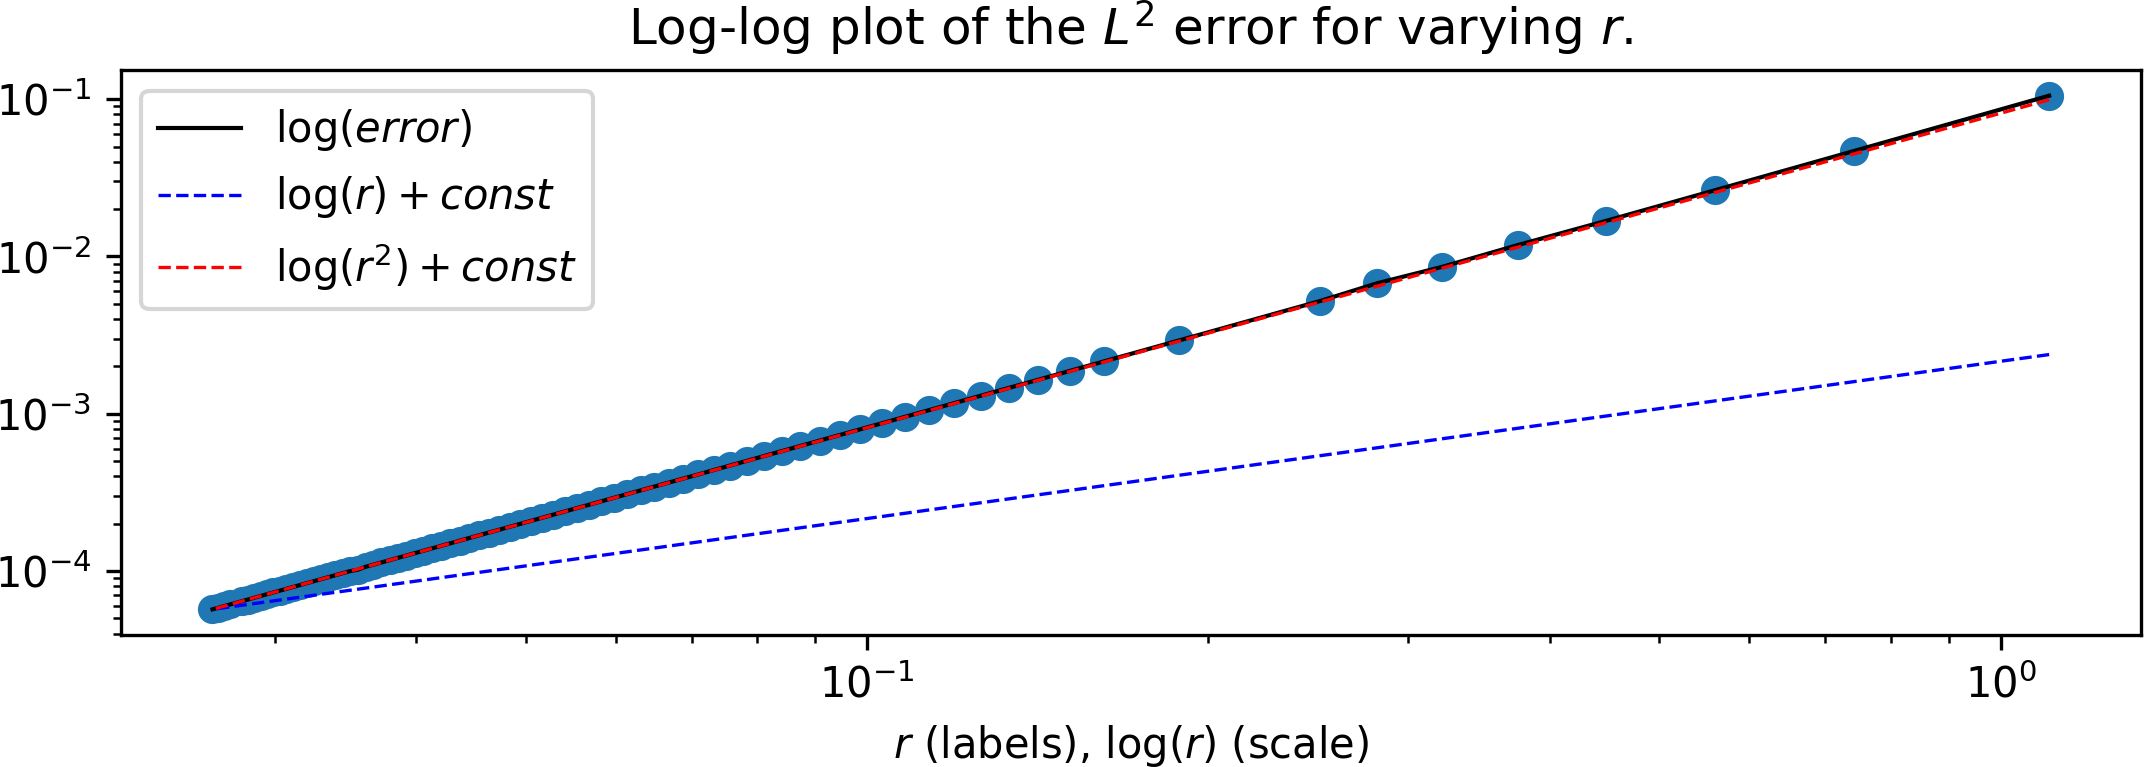
\includegraphics[width=1\linewidth]{figures/graphs/error_metric_file_square_fixup.png}
    \end{center}
    \caption{
        The $L^2$-norm error for the test problem \eqref{fvm_test_equation_1}, as parameter $r$ varies.
    }
    \label{error_fvm_1}
\end{figure}


We should also try a test problem which does not degenerate to Laplace's equation. Suppose instead that the exact solution is
$$
    h = e^{-2(x^2 + y^2)}.
$$
The source term $g$ is solved for as
$$
    -\Delta\left(e^{-2(x^2 + y^2)}\right) = g \quad \Rightarrow \quad g = \left(8 - 16x^2 - 16y^2\right)e^{-2(x^2 + y^2)},
$$
giving the new test problem,
\begin{equation}\label{fvm_test_equation_2}
    -\Delta h = \left(8 - 16x^2 - 16y^2\right)e^{-2(x^2 + y^2)},
    \quad \left.h\right|_\Gamma = e^{-2(x^2 + y^2)} \quad \text{(The test problem)}.
\end{equation}
The log-log error plot is displayed in figure \eqref{error_fvm_2}. In this case, there is still a clear quadratic convergence,
but with some oscillation in quality as $r$ decreases.
This is likely due to the coarse numerical integration of the heat source (which is using the rectangle rule for simplicity).
A visualization of these convergence results for problem \eqref{fvm_test_equation_2} is given in figure \ref{fvm_error_page}.
To emphasize the generality of the algorithm, figure \ref{fvm_laplace_error} displays convergence for problem \eqref{fvm_test_equation_1}
on an irregularly-meshed disk.

\begin{figure}[H]
    \begin{center}
        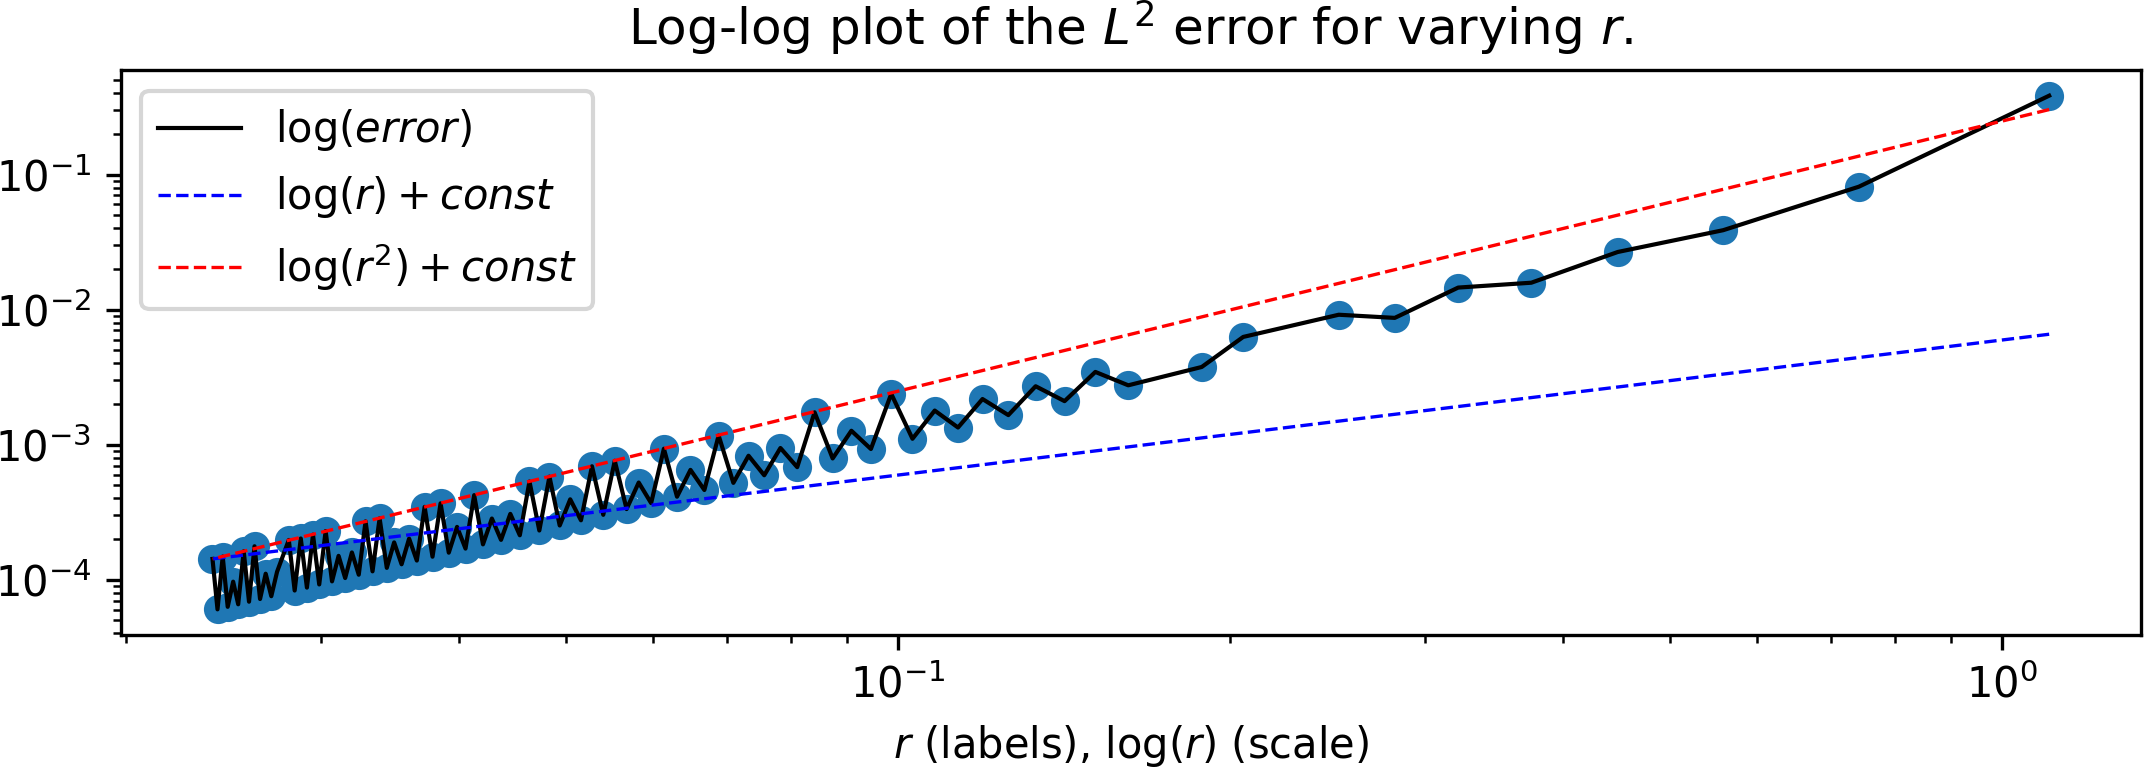
\includegraphics[width=1\linewidth]{figures/graphs/error_metric_file_square_2_fixup.png}
    \end{center}
    \caption{
        The $L^2$-norm error for the test problem \eqref{fvm_test_equation_2}, as parameter $r$ varies.
    }
    \label{error_fvm_2}
\end{figure}



\begin{figure}[H]
    \begin{center}
        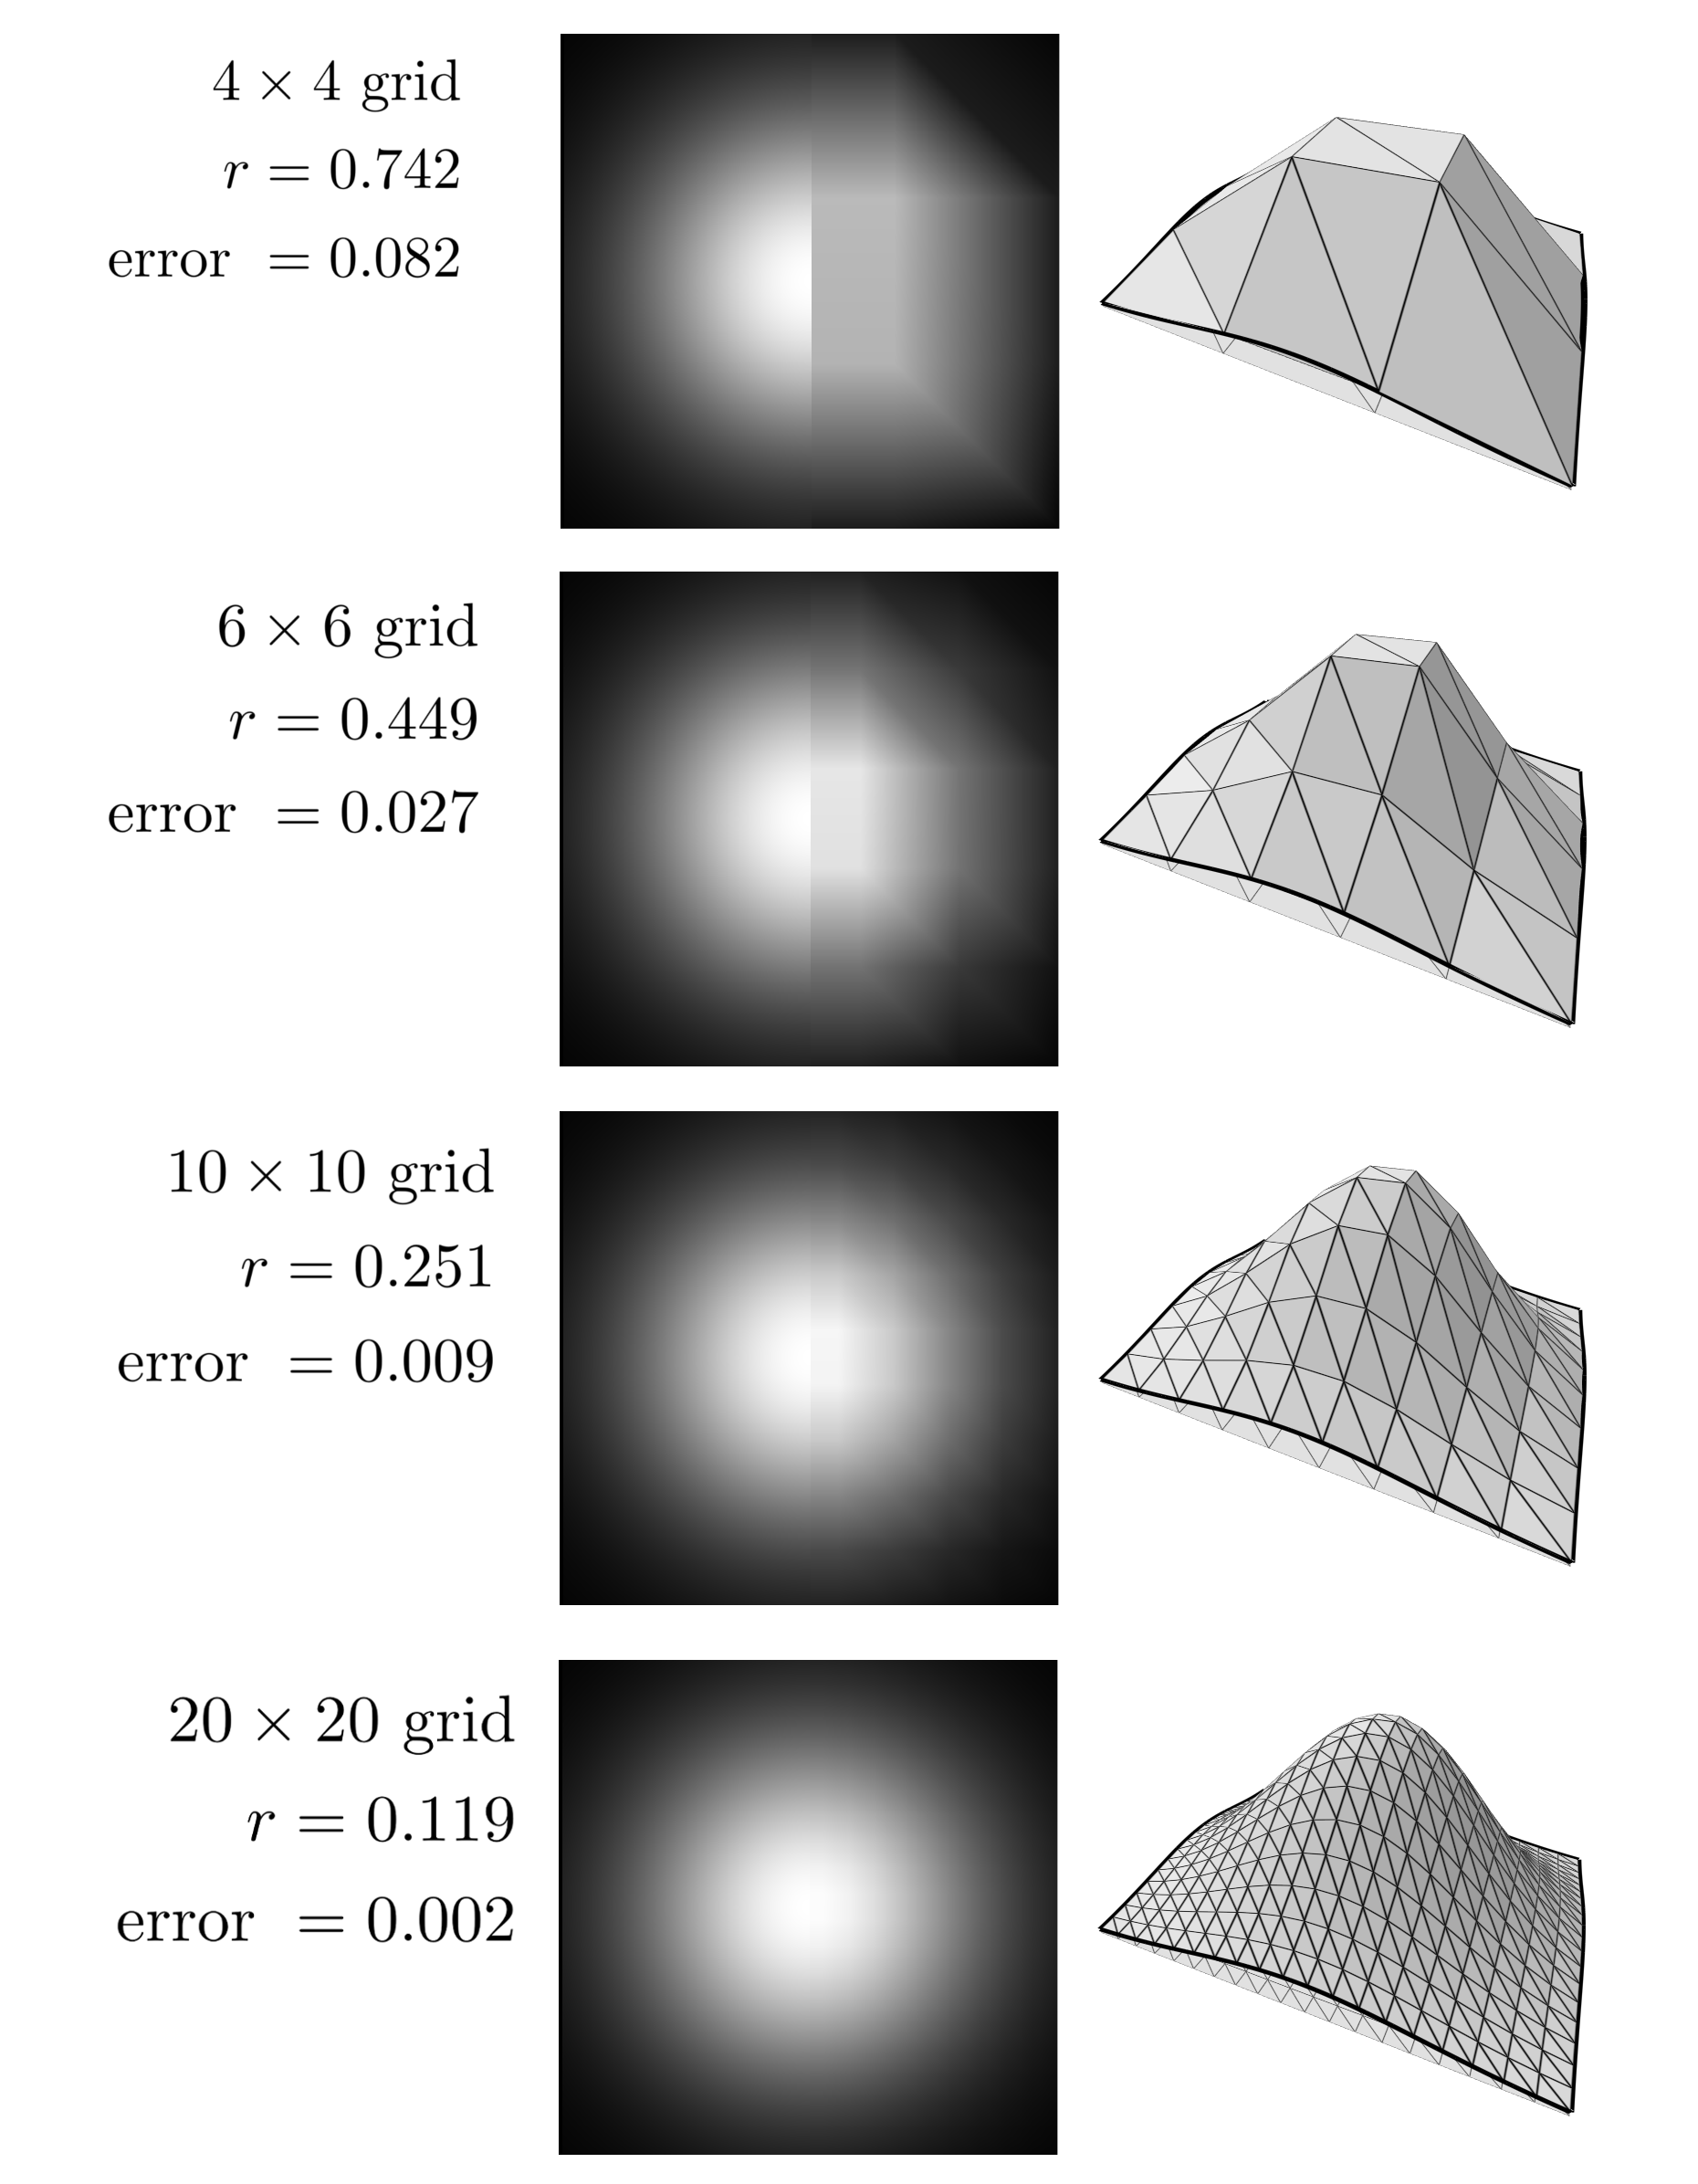
\includegraphics[width=1\linewidth]{figures/error/error.png}
    \end{center}
    \caption{
        Approximate solutions to the test problem \eqref{fvm_test_equation_2} with varying $r$.
        The middle squares contain plots of the exact solution (on the left rectangle), and the approximate solution (on the right rectangle).
        Black is $h = 0$, and white is $h = 1$.
        On the right, a 3D view of the solution and mesh is shown.
    }
    \label{fvm_error_page}
\end{figure}


\begin{figure}[H]
    \begin{center}
        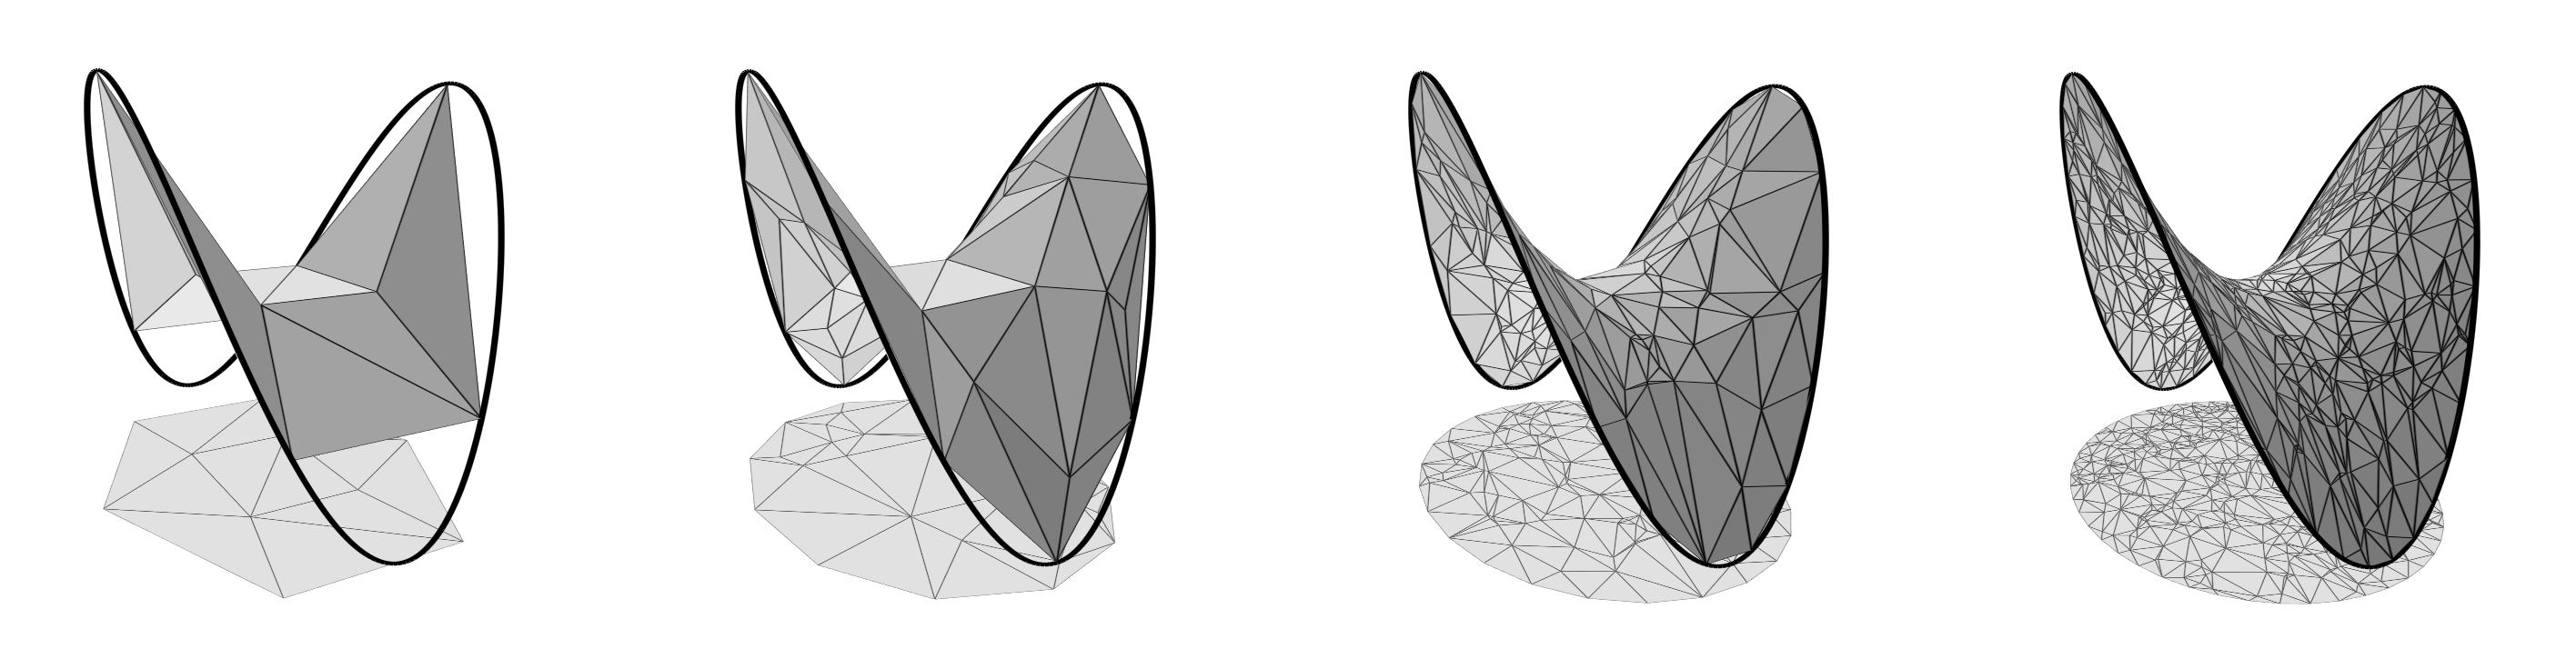
\includegraphics[width=1\linewidth]{figures/error/laplace_error.png}
    \end{center}
    \caption{
        Approximate solutions to the test problem \eqref{fvm_test_equation_1} with varying $r$.
        The domain is a unit disk, and $r$ is reduced by introducing random points. The finite volume algorithm \ref{alg:fvm}
        works trivially with curved domains and irregular meshes.
    }
    \label{fvm_laplace_error}
\end{figure}

% In geometry processing this matrix is called the ``cotangent Laplacian'' \cite{polygon_mesh_processing}, and it is typically
% applied to surface meshes in $\mathbb{R}^3$, which can be thought of as triangulations of a smooth surface.
% \subsection{Results and visualisation}
% \vskip 0.2in
% (results and visualisation)
% \vskip 0.2in
% We have worked through an instance of a \textit{finite volume method} \cite{pde_larsson}.
% Finite volume methods are characterised by a selection of a finite number of control volumes, and computation of flux integrals.
% Finite volume methods are typically \textit{conservative}, due to the ``flux network'' nature of the discretisation.

\section{From finite volumes to general Galerkin methods}
We will soon derive another instance of a Galerkin method, called a \textit{finite element method}.
This approach is directly related to the ``finite volumes'' described above. 
The finite element method, however, requires a construction called the \textit{weak form} of a PDE,
which can be directly motivated from the preceding discussion on finite volumes.
While each finite volume
has a clear geometric meaning (as a small cell around which a certain test flux integral is taken), the geometric meaning of a ``finite element''
requires slightly more thought, although it will be seen to be the same idea in disguise --- the resulting linear system
will be formed from averaged, or ``blurred'' flux integrals, rather than single flux integrals.
% Much of the resulting algorithm is the same as the finite volume method derived above, but
% with different integrals.

\subsection{Generalising the flux integrals by combining equations}

The matrix equation \eqref{poisson_matrix_equation} consists of linear equations
\begin{align*}
    \oint_{\pom_1} -\nabla \left(\sum_{i=1}^n h_i\phi_i\right) \cdot \hat{n}\,dx
    =
    \int_{\om_1}g\,dx\quad\text{(for $j=1$)},
\end{align*}
and so on. We cannot compute flux integrals
over all arbitrary control volumes, but we can take a number of ``trial'' flux integrals over the finite number of cells $\Omega_1,\cdots,\Omega_n$.
As with any linear system, we can take linear combinations of these equations to get more equations which must hold on a solution.
For example,
\begin{equation}\label{example_trial_sum}
    5\left[\oint_{\pom_1} -\nabla \left(\sum_{i=1}^n h_i\phi_i\right) \cdot \hat{n}\,dx\right]
    -
    2\left[\oint_{\pom_2} -\nabla \left(\sum_{i=1}^n h_i\phi_i\right) \cdot \hat{n}\,dx\right]
    =
    5\left[\int_{\om_1}g\,dx\right]
    -
    2\left[\int_{\om_2}g\,dx\right]
\end{equation}
must hold for a solution $\hat{h}$ to \eqref{poisson_matrix_equation}.
Equation \eqref{example_trial_sum} is not a flux integral, but a sum of flux integrals.
Now suppose instead we are working with the original integral form of Poisson's equation, \eqref{poisson_equation_integral}:
\begin{equation*}
    \oint_{\pomn} -\nabla h\cdot \hat{n}\,dx = \int_{\omn} g\,dx \quad \text{for all control volumes $\Omega_0$.}
\end{equation*}
Then, in the same way, we can take linear combinations of the equations \eqref{poisson_equation_integral}
for some collection of control volumes, to get another equation which the exact solution $h$ must satisfy. In addition we can take integral
combinations, whenever that integral is well-defined. For example, consider a parameterised family of control volumes,
$\left\{\Omega_{0,t} \mid 0 < t  < 1\right\}$, defined by
    $$\Omega_{0,t} = \text{the disk of radius $t$ around some fixed point $c$}.$$
Then the equation
\begin{equation}\label{poisson_integral_example}
    \int_{t=0}^{t=1}\left[\oint_{\partial\Omega_{0,t}} -\nabla h\cdot \hat{n}\,dx\right]\,dt = \int_{t=0}^{t=1}\left[\int_{\Omega_{0,t}} g\,dx\right]\,dt
\end{equation}
must also hold for the exact solution $h$. We therefore have an alternative route to discretization of the integral equation \eqref{poisson_equation_integral}:
instead of choosing a finite number of flux equations over single control volumes, we choose a finite number of integrals of flux equations over
families of control volumes.

\subsection{The weak form of Poisson's equation}
The averaged flux integral equation \eqref{poisson_integral_example}, expressed as a nested integral, can be restated as a single integral over
the whole domain:
\begin{equation}\label{poisson_integral_example_modified}
    \int_{\Omega}\nabla h\cdot \nabla v\,dx = \int_{\Omega}gv\,dx,
\end{equation}
where $v$ is a scalar function defined as
\begin{equation}\label{poisson_integral_example_v}
    v(x) = 
    \left\{\begin{array}{lr}
        1 - t &\text{if $x \in \Omega_{0,t}$}\\
        0 &\text{otherwise}.\\
        \end{array}\right.
\end{equation}
This deserves some explanation, which will be given at two levels of informality.
The concentric family of control volumes $\Omega_{0,t}$ appear as level sets $v = 1-t$.
Since this cone has unit slope, the normal $\hat{n}$ of the level set $v = 1-t$ is $-\nabla v$. Since the left-hand side of
\eqref{poisson_integral_example_modified} is an integral over the fluxes through each level set, the nested integral is subsumed into
one integral over the union of level sets.
The outer integral of the right-hand side of \eqref{poisson_integral_example_modified} consists of a ``stack of integrations'' of $g$ against concentric disks, which 
is equivalent to integrating $g$ against a ``stack of concentric disks'', or rather, the cone $v$ \eqref{poisson_integral_example_v}.

\vskip 0.2in
(draw this)
\vskip 0.2in

At another level of informality, with more notation, we can define the indicator function
\begin{equation}\label{fem_indicator_function}
    \chi(\Omega_{0,t})(x) = 
    \left\{\begin{array}{lr}
        1 &\text{if $x \in \Omega_{0,t}$}\\
        0 &\text{otherwise},\\
        \end{array}\right.
\end{equation}
and define the gradient of the indicator function by
\begin{equation}\label{fem_indicator_gradient}
    \nabla\chi(\Omega_{0,t})(x) = 
    \left\{\begin{array}{lr}
        -\hat{n}\cdot\infty &\text{if $x \in \pom_{0,t}$}\\
        0 &\text{otherwise}.\\
        \end{array}\right.
\end{equation}
The $\infty$ is an informal way of stating that a 2D integral will give a non-zero value on this boundary,
which is a set of measure zero --- with typical functions, any isolated set of measure zero is ignored
\footnote{This idea (and the related
Dirac delta ``function'') is formalised in
the theory of distributions, or generalised functions, introduced by Laurent Schwartz in the late 1940s.}.
If there should be any definition of a ``generalised gradient'', this seems reasonable --- if the indicator function
$\chi(\Omega_{0,t})$ is approximated by a sequence of smooth functions $f_1, f_2,\ldots$, the gradient $\nabla f_i$
will approach \eqref{fem_indicator_gradient}.

\vskip 0.2in
(draw this)
\vskip 0.2in

We then have the equalities
\begin{align*}
    \int_{t=0}^{t=1}\left[\oint_{\partial\Omega_{0,t}} -\nabla h\cdot \hat{n}\,dx\right]\,dt
    &= \int_{t=0}^{t=1} \left[
        \int_\Omega \nabla h\cdot \nabla \chi(\Omega_{0,t})\,dx
    \right]\,dt
    \\
    &= \int_\Omega \nabla h \cdot \nabla \left[
        \int_{t=0}^{t=1}\chi(\Omega_{0,t})\,dt
    \right]\,dx,
\end{align*}
where the final equality might assume some regularity (--- Fubini's theorem?).
We then define
\begin{equation}\label{fem_v_definition}
    v \coloneqq \int_{t=0}^{t=1}\chi(\Omega_{0,t})\,dt,
\end{equation}
which is simplified to \eqref{poisson_integral_example_v}.
Note that $\nabla v$ is not defined everywhere ($\nabla v$ does not exist at $c$ or on the unit circle around $c$).
However, this is fine, as these are isolated sets of measure zero, which can be ignored as making no contribution to the integral.
Formally, $v$ is in the Sobolev space $H^1_0(\Omega)$, where the $0$ subscript denotes
that $v$ must vanish on the boundary $\Gamma$. (The integral of fluxes cannot contain a flux measurement
across $\Gamma$, as the solution there is specified by the Dirichlet boundary condition --- there is no flux information on $\Gamma$.)

Now we can forget our specific definition of $v$, and define the \textit{weak form} of Poisson's equation to be
\begin{equation}\label{poisson_equation_weak_form}
    \int_\Omega \nabla h \cdot \nabla v \,dx = \int_\Omega gv\,dx \text{\quad for all $v \in H^1_0(\Omega)$}.
\end{equation}
The weak form will be the starting point for deriving general Galerkin methods.

\subsection{General Galerkin methods for Poisson's equation}
A general Galerkin method will discretize the test space as usual, approximating $h$ by
$$\tilde{h} \in \Phi = \text{span}\left\{\phi_1, \cdots, \phi_n\right\},$$
and will also approximate the ``trial space'' $H^1_0(\Omega)$
\footnote{The function space $\Psi$ is called the trial space as it determines the finite number of ``trial equations'' which need to hold in order
           to establish that $\tilde{h}$ is an approximate solution.}
as
    $$v \in \Psi = \text{span}\left\{\psi_1, \cdots, \psi_n\right\}.$$
Since the weak form equations \eqref{poisson_equation_weak_form} are linear in $v$, we need only check them for $v=\psi_1,\cdots,\psi_n$.
The resulting discrete system of equations for a general Galerkin method is
\begin{equation}\label{poisson_galerkin_system}
\begin{split}
    \int_\Omega \nabla\tilde{h}\cdot \nabla\psi_j\,dx
        &\equiv \int_\Omega \nabla(\phi_\Gamma + \Phi\cdot\hat{h})\cdot \nabla\psi_j\,dx \\
    &\equiv \int_\Omega \nabla\phi_\Gamma \cdot \nabla\psi_j\,dx + \sum_{i=1}^n h_i\int_\Omega \nabla\phi_i\cdot \nabla\psi_j\,dx\\
    &= \int_\Omega g\psi_j\,dx,
        \text{\quad\quad $j = 1,\cdots,n$}.
\end{split}
\end{equation}
Remember that we start with the discrete solution space $\Phi^*$, then define the test space $\Phi$ to be $\Phi^*$ restricted to those functions vanishing on $\Gamma$.
The term $\phi_\Gamma \in \Phi^*$ is a ``base'' term which approximates the boundary condition $h_\Gamma$ on $\Gamma$.
We can try just about any kind of function spaces for $\Phi$ and $\Psi$, but we can make some broad distinctions, for example:
\begin{itemize}
    \item If $\Psi = \Phi$, then we call this a \textit{Bubnov--Galerkin} method.
    \item If $\Psi \neq \Phi$, then we call this a \textit{Petrov--Galerkin} method.
\end{itemize}
Further, whether Bubnov-- or Petrov--Galerkin, there are two common classes of $H^1_0$-conforming Galerkin methods:
\begin{itemize}
    \item If the $\Phi$ and $\Psi$ basis functions have well-localised compact support, we get the \textit{finite element method}.
    \item If the $\Phi$ and $\Psi$ basis functions are non-localised global functions, for example harmonics of $\Omega$, we get the \textit{spectral method}.
\end{itemize}
Next, we will derive a simple finite element method for Poisson's equation.

\begin{aside}
Relation to FVM: The finite volume method can be considered a sharp edge case of \eqref{poisson_galerkin_system}, where $\Psi_{\text{FVM}}$ is defined as
$$
    \Psi_{\text{FVM}} = \text{span}\left\{\chi(\Omega_1), \cdots, \chi(\Omega_n)\right\}
$$
for some choice of control volumes $\Omega_1, \cdots, \Omega_n$.
While $\Psi_{\text{FVM}}$ is technically not $H^1_0$-conforming, if the gradient generalisation \eqref{fem_indicator_gradient} is used, the result is the finite volume method.
\end{aside}





% At first sight, \eqref{example_trial_sum} cannot directly be interpreted as a statement about a ``flux integral'', but rather about a sum
% of flux integrals. However, a key idea is to regard \eqref{example_trial_sum} as a flux integral over a \textit{formal sum} of domains,
%     $$\Omega_1 + \Omega_2.$$
% We now have the equation
% \begin{equation}
%     \int_{\pom_1 + \pom_2} -\nabla \left(\sum_{i=1}^n h_i\phi_i\right) \cdot \hat{n}\,dx
%     =
%     \int_{\om_1 + \om_2}g\,dx.
% \end{equation}
% In differential geometry $\Omega_1 + \Omega_2$ is called a \textit{chain}. For example, we may visualise $\Omega_1 + 2\Omega_2 + 0.5\Omega_4$ as:
% 
% \vskip 0.2in
% (draw this)
% \vskip 0.2in
% 
% We define the boundary operator $\partial$ to be linear in formal sums e.g.,
%     $$\partial(\Omega_1 + \Omega_2) = \pom_1 + \pom_2.$$
% If $\om_1$ and $\om_2$ share a boundary, we would like $\om_1 + \om_2$ to represent their union, such that a flux
% integral over $\partial(\Omega_1 + \Omega_2)$ evaluates to zero on the shared boundary. This can be done by thinking of
% the boundary as \textit{oriented}, as in, consisting of oriented ``surface elements'' over which flux integrals can be taken.
% For example, the $\hat{n}$ in a flux integral denotes the outward-pointing normal, which represents an ``outward-flux-measuring surface element''.
% The opposite $-\hat{n}$ then represents the ``inward-flux-measuring surface element'', which is outward from the perspective of an adjacent cell.
% 
% \vskip 0.2in
% (draw this)
% \vskip 0.2in
% 
% We may now define
%     $$\Psi = \text{span}\left\{\Omega_1,\cdots,\Omega_n\right\}$$
% to be the \textit{trial space}, where the span is taken with respect to formal sums. As with a typical linear space,
% we may choose from many possible bases. For example,
%     $$\Psi = \text{span}\left\{\Omega_1, \Omega_2, \Omega_3\right\} =
%     \text{span}\left\{\Omega_1 + \Omega_2, 2\Omega_2, \Omega_3\right\}.$$
% A key idea, leading to Galerkin methods, is to allow freedom in the choice of the trial space $\Psi$.
% Notably, we do not need $\Psi$ to be a space of formal sums of domains.
% The Poisson equation is discretised over flux integrals around cell boundaries in the linear system \eqref{poisson_equation_integral_discretized},
% which we repeat here:
% \begin{align*}
%     \sum_{i=1}^n h_i\int_{\pom_j} -\nabla \phi_i \cdot \hat{n}\,dx = \int_{\om_j} g\,dx,\quad j=1,\cdots,n.
% \end{align*}
% Applying Stokes' theorem, we get
% \begin{align*}
%     \sum_{i=1}^n h_i\int_{\om_j} -\Delta \phi_i \,dx = \int_{\om_j} g\,dx,\quad j=1,\cdots,n.
% \end{align*}
% We can think of these integrals as over the \textit{entire domain} $\Omega$, giving the form
% \begin{align*}
%     \sum_{i=1}^n h_i\int_{\om} -\Delta \phi_i\cdot \chi(\om_j)\,dx = \int_{\om} g\cdot\chi(\om_j)\,dx,\quad j=1,\cdots,n.
% \end{align*}
% where $\chi(\om_j)$ is the indicator function of $\om_j$,
% \begin{align*}
%     \chi(\om_j)(x) \coloneqq \left\{\begin{array}{lr}
%         0 &\text{if $x \in \om_j$}\\
%         1 &\text{if $x \notin \om_j$.}\\
%         \end{array}\right.
% \end{align*}
% We can now think of our trial space $\Psi$ as a span of functions, instead of a span of domains:
%     $$\Psi = \text{span}\left\{\chi(\Omega_1),\cdots,\chi(\Omega_n)\right\}.$$
% Now, as the trial space is just a regular function space, we could instead let
%     $$\Psi = \text{span}\left\{\psi_1,\cdots,\psi_n\right\}$$
% where the $\psi_j$
% need not be the indicator functions of a selection of control volumes. We now have the system of equations
% \begin{align*}
%     \sum_{i=1}^n h_i\int_{\om} -\Delta \phi_i \psi_j\,dx = \int_{\om} g\psi_j\,dx,\quad j=1,\cdots,n.
% \end{align*}
% By integration by parts we have the system of equations
% \begin{equation}\label{poisson_galerkin}
%     \sum_{i=1}^n h_i\int_{\om} \nabla \phi_i \cdot \nabla \psi_j\,dx = \int_{\om} g\psi_j\,dx,\quad j=1,\cdots,n,
% \end{equation}
% and we see that we still only require the $\phi_i$ to be in $H^1(\Omega)$.
% We can see that equation \eqref{poisson_galerkin} is very similar to the exact fluxes in \eqref{poisson_equation_integral_discretized},
% and indeed \eqref{poisson_galerkin} gives a discrete linear system in much the same way.
% There is a real geometric sense in which \eqref{poisson_galerkin} is a ``blurred convolution'' of flux integrals.
% 
% --- Mention the weak form, the above is an alternative motivation using the discrete equations rather than
% variational methods with the original PDE.

% \subsubsection{Integrating over trial functions versus integrating over domains}
% The above construction (generalising a finite volume flux integral to a finite-element ``blurred flux'' integral) is further investigated
% below.
% We will work with the Dirac delta ``function'' (which is rather a distribution, or generalised function),
% defined by
% \begin{align*}
%     \int_{\omn} \delta_y\,dx = 
%     \left\{\begin{array}{lr}
%         1 &\text{if $y \in \omn$}\\
%         0 &\text{otherwise}.\\
%         \end{array}\right.
% \end{align*}
% For example, possibly under some regularity assumptions, we may represent a trial function $\psi_j$ on $\Omega$ as
%     $$f = \int_\Omega \delta_x f(x)\,dx,$$
% which could be called ``Riemann-integral-like''.
% We may instead represent $\psi_j$ in a ``Lebesgue-integral-like'' way by defining
%     $$L_y(\psi_j) \coloneqq \left\{z \in \Omega \mid \psi_j(z) = y\right\}$$
% to be a level set of $\psi_j$, the points of $\Omega$ for which $\psi_j = y$. We can then express $\psi_j$ as
%     $$\psi_j = \int_{-\infty}^\infty \left[\int_{L_y(\psi_j)} y\delta_x \,dx\right]\,dy.$$
% This gives $\psi_j$ as the totality of its level sets.
% For example, if we let $\Psi$ be spanned by the hat functions on some triangulation, each hat function $\psi_j$
% can be thought of as a totality of level sets culminating in the point-set of $\psi_j(p_j) = 1$.
% 
% \vskip 0.2in
% (draw this)
% \vskip 0.2in
% 
% The discretised Poisson equation \eqref{poisson_galerkin} involves an integral over $\nabla \phi_i \cdot \nabla \psi_j$,
% and we can compute this as
% \begin{equation}\label{flux_convolution}
% \begin{split}
%     \int_{\om} \nabla \phi_i \cdot \nabla \psi_j\,dx
%         &= \int_{-\infty}^\infty \int_{\om} \nabla\phi_i \cdot \nabla\left[\int_{L_y(\psi_j)} y\delta_z \,dz\right]\,dx\,dy\\
%         &= \int_{-\infty}^\infty y \int_{L_y(\psi_j)} \nabla\phi_i \cdot \hat{n}\,dx\,dy.
% \end{split}
% \end{equation}
% We have this final equality by noting that the gradient of $\psi_j$ at $x$, where $\psi_j(x) = y$, is orthogonal to the level set $L_y{(\psi_j)}$,
% and has length $y$:
% 
% \vskip 0.2in
% (draw this)
% \vskip 0.2in
% 
% We can think of the ``flux trial'' \eqref{poisson_galerkin} as involving ``blurred fluxes'' as in \eqref{flux_convolution}.
% For example, if we let $\Phi = \Psi$ be the set of hat functions on some triangulation
% of $\Omega$, then form and solve the matrix system, we get a generally non-conservative system of fluxes. We have lost conservativeness
% by the ``blurring'' of the flux integrals, but we may have gained advantages in terms of stability and convergence: in this case,
% the linear system will be symmetric-positive-definite, and stably solvable by, for example, conjugate gradients.

\section{Discretizing Poisson's equation by finite elements}
We now derive two finite element methods for Poisson's equation. The first will use
the same piecewise linear triangulation scheme as for the previous FVM, but with seemingly different integrals --- the
result will turn out to not give any improvement over algorithm \ref{alg:fvm}. However, we will subsequently generalise this finite element method
to a higher order method.

\subsection{Forming a linear system}
We now start with the weak form \eqref{poisson_equation_weak_form}.
Firstly, we can express the resulting Galerkin linear system in matrix form as

\renewcommand{\integralentry}[2]{\int_{\om}\nabla\phi_{#2}\cdot\nabla{\psi_j}\,dx}
\renewcommand{\integralrhsentry}[1]{\int_{\om}g\psi_j\,dx - \int_{\om}\nabla\phi_\Gamma\cdot\nabla{\psi_j}\,dx}
\begin{equation}\label{fem_poisson_matrix_equation}
\begin{split}
    A\hat{h}
    &= \begin{bmatrix}
            \integralentry{1}{1} & \cdots & \integralentry{1}{n} \\
            \vdots & & \vdots \\
            \integralentry{n}{1} & \cdots & \integralentry{n}{n}
    \end{bmatrix}
    \begin{bmatrix} h_1 \\ \vdots \\ h_n \end{bmatrix}
    \\
    &= \begin{bmatrix} \integralrhsentry{1} \\ \vdots \\ \integralrhsentry{n}  \end{bmatrix}
    = \hat{f}.
\end{split}
\end{equation}
This is much the same as the FVM matrix equation \eqref{poisson_matrix_equation}, with flux integrals replaced
by integrals against trial functions (giving ``blurred'' flux integrals).
Notice that the integrals in \eqref{fem_poisson_matrix_equation}, in contrast to \eqref{poisson_matrix_equation},
are over the \textit{entire domain}. It may be very costly in general to construct such a matrix, requiring
the computation of many large integrals. The finite element method, in particular, solves this problem
by ``localising'' basis functions of the test and trial spaces. Each basis test function $\phi_i$
has \textit{compact support}, meaning that there is some compact subdomain $D^\phi_i$ such that
\begin{align*}
    \phi_i(x) =
    \left\{\begin{array}{lr}
        \phi_i(x) &\text{if $x \in D^\phi_i$}\\
        0 &\text{otherwise},\\
    \end{array}\right.
\end{align*}
and similarly each basis trial function $\psi_i$ has some corresponding compact subdomain $D^\psi_i$ such that
\begin{align*}
    \psi_i(x) =
    \left\{\begin{array}{lr}
        \psi_i(x) &\text{if $x \in D^\psi_i$}\\
        0 &\text{otherwise}.\\
    \end{array}\right.
\end{align*}
This has the effect of reducing the domain of each integral in \eqref{fem_poisson_matrix_equation}, as
    $$\int_\Omega \nabla\phi_i \cdot \nabla\psi_j\,dx = \int_{D_i^\phi \cap D_j^\psi} \nabla\phi_i \cdot \nabla\psi_j\,dx. $$
With well-localised basis functions, the intersection will be
    $$D_i^\phi \cap D_j^\psi = \emptyset$$
for most indices $i,j$, implying the matrix \eqref{fem_poisson_matrix_equation} will be \textit{sparse}. In practice this allows
the use of iterative or graph-based sparse matrix algorithms which can be hugely more efficient than dense matrix computations of the same size.
The size of the matrix will increase quadratically with the number of nodes in the discretization, while the number of nonzeros
typically increases linearly.
A typical sparsity pattern for a finite element problem is shown in figure \ref{sparsity_pattern}.

\begin{figure}[H]
    \begin{center}
        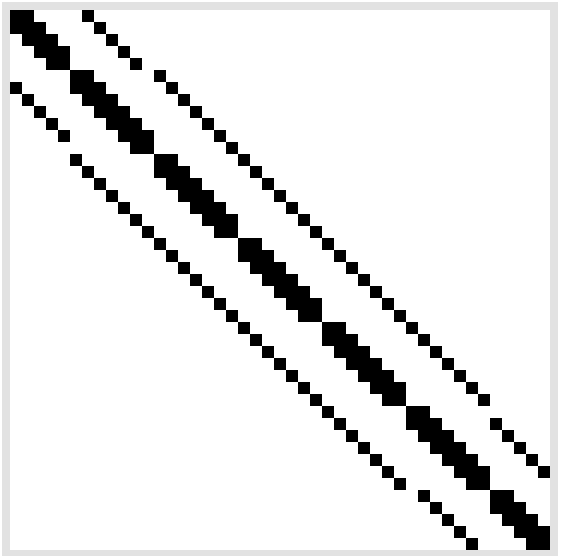
\includegraphics[width=0.26\linewidth]{figures/sparsity_pattern_no_text.png}
    \end{center}
    \caption{\scriptsize
        An example sparsity pattern for the finite element matrix of a 2D Poisson problem. White is zero and black is non-zero.
        The mesh has 61 vertices (16 on the boundary), and 104 triangles, resulting in a 45x45 system with 2025 entries, 197 non-zeros, and fill of $0.0973$.
    }
    \label{sparsity_pattern}
\end{figure}

\subsection{A piecewise linear finite element triangulation scheme}
We can use almost the same piecewise linear triangulation scheme as in the finite volume method, but we no longer
take trial flux integrals over mixed Voronoi cells. Instead, we can use the Bubnov--Galerkin method: Let $\Psi = \Phi$
(which are the hat functions) and form the system of linear equations \eqref{poisson_galerkin_system}.
\subsubsection{Computing the linear system by closed form integration}\label{fem_closed_form}
In deriving the FVM, we had to compute closed form flux integrals over complex polygonal cells.
At first sight, the integration required for our new FEM method is different, although many of the steps here are the same as
in section \ref{fvm_closed_form}. However, the integrals for the matrix system \eqref{poisson_galerkin_system} will turn out to be
\textit{exactly} the same as those derived for our finite volume method. This is a peculiarity of the hat functions --- we will then
show how this, seemingly pedantic, complete derivation of this equivalent FEM scheme, can be generalised.

Again, we use the piecewise linear interpolation \eqref{boundary_approximation} of the Dirichlet boundary function $h_\Gamma$:
\begin{equation*}
    \phi_\Gamma = h_\Gamma(p^\Gamma_1)\hatfun{p^\Gamma_1}
                + \cdots
                + h_\Gamma(p^\Gamma_{n_\Gamma})\hatfun{p^\Gamma_{n_\Gamma}}.
\end{equation*}
As before, we expand the gradient $\nabla\tilde{h}$ \eqref{gradient_expansion} by linearity as
\begin{equation*}
    \nabla \tilde{h} = \nabla\phi_\Gamma + \nabla\phi
             = \sum_{i=1}^{n_\Gamma}h_\Gamma(p^\Gamma_i)\nabla\phi^\Gamma_i + \sum_{i=1}^n h_i\nabla\phi_i,
\end{equation*}
and in this case the (Bubnov--)Galerkin linear system \eqref{poisson_galerkin_system} becomes
\begin{equation}\label{fem_integral_linearity_expanded}
    \int_{\om} \nabla \tilde{h}\cdot \nabla \phi_j\,dx
    =
    \sum_{i=1}^{n_\Gamma}\left[h_\Gamma(p^\Gamma_i)\int_{\om}\nabla\phi^\Gamma_i\cdot\nabla\phi_j\,dx\right]
    + \sum_{i=1}^n\left[h_i\int_{\om}\nabla\phi_i\cdot\nabla\phi_j\,dx\right].
\end{equation}
As in section \ref{fvm_closed_form}, we now reexpress \eqref{fem_integral_linearity_expanded} in terms of local indices. First, note that a trial function
$\psi_j = \phi_j$ has compact support, with domain $D^\phi_j = D^\psi_j = D_j$,
which is the union of triangles incident to the interior vertex $p_j$.
This domain intersects with the domains of those hat basis functions of $\Phi^*$ which are centred on $p_j$ or an adjacent vertex
(either in the interior or on the boundary).
We will compute the integral for a certain trial function $\psi = \psi_j$.
We repeat the local index definitions from section \ref{fvm_closed_form} here.
\definelocalterms{the trial function $\psi = \psi_j = \phi_j$}
The local form of the equation \eqref{fem_integral_linearity_expanded} is then

\begin{equation}\label{fem_integral_vertex}
    \int_{\om} \nabla \tilde{h}\cdot \nabla \psi\,dx
     = h_j\int_{\om}\nabla\phi_v\cdot\nabla\psi\,dx + \sum_{l=1}^{k}h_{v_l}\int_{\om}\nabla\phi^v_l\cdot\nabla\psi\,dx,
\end{equation}
where, as in \ref{fvm_closed_form}, $h_{v_i}$ is defined as
\hvidefinition
Again, with the same reasoning as in section \ref{fvm_closed_form}, due to $\nabla\phi_i = \nabla\psi_i$ being constant on each triangle, to simplify integration
we break \eqref{fem_integral_vertex} into a sum of integrals over triangles:
\begin{equation}\label{fem_integral_vertex_triangles}
    \int_{\om} \nabla \tilde{h}\cdot \nabla \psi\,dx
    = \sum_{t=1}^k\left[\int_{T^v_t}\nabla\phi_v\cdot\nabla\psi\,dx + \sum_{l=1}^{k}h_{v_l}\int_{T^v_t}\nabla\phi^v_l\cdot\nabla\psi\,dx\right].
\end{equation}
We want to reduce an integral over each separate triangle (oblique, isosceles, etc.) to an integral over a reference triangle
for which we have closed forms.
This is a common pattern in the finite element method.
We will transform each triangle domain $T$ into a ``reference element''
% % Right angled triangle.
% % https://tex.stackexchange.com/questions/65455/is-there-a-math-symbol-for-right-angled-triangle
% \def\ll{{\mbox{\begin{picture}(7,10)
% \put(1,0){\line(1,0){5}}
% \put(6,0){\line(-1,2){5}}
% \put(1,0){\line(0,1){10}}
% \end{picture}
% }}}
\newcommand{\reftri}{{\mathcal{R}}}
$\reftri$, defined by
    $$\reftri = \left\{(x,y) \in [0,1]^2 \mid x + y < 1\right\}.$$
We introduce the ``reference basis functions'', which account for all possible ways a hat function could intersect with this triangle:
\begin{equation}\label{fem_reference_basis_functions}
    \Phi^\reftri_1 = 1-x-y, \text{\quad and \quad} \Phi^\reftri_2 = x \text{\quad and \quad} \Phi^\reftri_3 = y.
\end{equation}
with gradients
\begin{equation}\label{fem_reference_basis_function_gradients}
    \nabla\Phi^\reftri_1 = (-1, -1)^T, \text{\quad and \quad} \nabla\Phi^\reftri_2 = (1,0)^T \text{\quad and \quad} \Phi^\reftri_3 = (0,1)^T.
\end{equation}

\vskip 0.2in
(draw $\reftri$ and reference basis functions)
\vskip 0.2in

Suppose we are computing the integral \eqref{fem_integral_vertex_triangles} around some interior vertex $v$,
and are computing the subintegral for some incident triangle $T$ with vertices $v,v^\pr,v^\ppr$.
We would like to make a change of variables to the reference domain $\reftri$.
The affine map
\newcommand{\affmap}{\gamma}
$\affmap : \reftri \rightarrow T$ defined by
\begin{equation}\label{fem_affine_map}
    \affmap(x,y) = v + (v^\pr - v)x + (v^\ppr - v)y
\end{equation}
gives a pullback of scalar functions $\Phi^\reftri_{1,2,3}$ on $\reftri$
to scalar functions $\Phi_{1,2,3}$ on $T$. These scalar functions on $T$ correspond
exactly to those pieces of basis hat functions whose gradients we want to integrate.

\vskip 0.2in
(draw this affine mapping)
\vskip 0.2in

To derive a change of variables formula, we need to compute the Jacobian matrix of $\affmap$:
$$
    J = \begin{bmatrix} \Part{\affmap_x}{x} & \Part{\affmap_x}{y} \\ 
                        \Part{\affmap_y}{x} & \Part{\affmap_y}{y} \end{bmatrix}
      =
        \left[
        \begin{array}{c|c}
            v^\pr - v & v^\ppr - v
        \end{array}
        \right].
$$
If we pushforward the domain of integration from $T$ to $\reftri$ by $\affmap$ (enacting a change of variables),
the resulting expression is
\begin{equation}\label{fem_closed_form_integral_complicated}
    \int_T \nabla\Phi_l \cdot \nabla\Phi_m\,dx
        = \int_\reftri \det(J)(J^{-T}\nabla\Phi^\reftri_l)\cdot(J^{-T}\nabla\Phi^\reftri_m)\,dx.
\end{equation}
Since $J$ depends only on the triangle vertex positions $v,v^\pr,v^\ppr$, it is constant on $\reftri$, and we can easily compute its inverse transpose
(using the standard $2 \times 2$ inverse formula):
\begin{align*}
    J^{-T} = \frac{1}{\det(J)}\begin{bmatrix}
        v_y^\ppr - v_y & v_y - v^\pr_y \\ v_x - v_x^\ppr & v^\pr_x - v_x
    \end{bmatrix}
    = \frac{1}{2\text{Area}(T)}\left[\begin{array}{c|c}
        (v - v^\ppr)^\perp & (v^\pr - v)^\perp
    \end{array}\right].
\end{align*}

Since the integrand is constant,
\eqref{fem_closed_form_integral_complicated} simplifies to
\begin{equation}\label{fem_closed_form_integral}
    \int_T \nabla\Phi_l \cdot \nabla\Phi_m\,dx
        = \text{Area}(T)(J^{-T}\nabla\Phi^\reftri_l)\cdot(J^{-T}\nabla\Phi^\reftri_m),
\end{equation}
and if we define the matrix
\begin{align*}
    K = \left[\begin{array}{c|c}
        (v - v^\ppr)^\perp & (v^\pr - v)^\perp
    \end{array}\right],
\end{align*}
the equation \eqref{fem_closed_form_integral} is further simplified to
\begin{equation}\label{fem_closed_form_integral_simple}
    \int_T \nabla\Phi_l \cdot \nabla\Phi_m\,dx
        = \frac{1}{4\text{Area}(T)} (K\nabla\Phi^\reftri_l)\cdot(K\nabla\Phi^\reftri_m).
\end{equation}
Plugging in the gradients \label{fem_reference_basis_function_gradients}, we get
\begin{equation}
    K\nabla\Phi^\reftri_1 = (v^\ppr - v^\pr)^\perp, \text{\quad and \quad}
    K\nabla\Phi^\reftri_2 = (v - v^\ppr)^\perp, \text{\quad and \quad}
    K\nabla\Phi^\reftri_3 = (v^\pr - v)^\perp.
\end{equation}
By plugging these expressions into \eqref{fem_closed_form_integral_simple}, we get
\begin{align*}
    \int_L \nabla\Phi_v\cdot\psi\,dx
        &= \frac{1}{4\text{Area}(T)}\norm{v_{t+1} - v_t}^2,\\
    \int_L \nabla\Phi_{v_t}\cdot\nabla\psi\,dx
        &= \frac{1}{4\text{Area}(T)}(v - v_{t+1})\cdot(v_{t+1} - v_t),\\
    \int_L \nabla\Phi_{v_{t+1}}\cdot\nabla\psi\,dx
        &= \frac{1}{4\text{Area}(T)}(v_t - v)\cdot(v_{t+1} - v_t).
\end{align*}
Note that these are the same as the closed forms \eqref{fvm_closed_form_integrals} derived for the finite volume method.
Now we notice that all this work has been wasted, as this finite element method gives
exactly the same matrix as the previous finite volume method.

\subsubsection{Integrating the source function}
Again, one more thing is needed.
We require some numerical integration for the right-hand side source terms
    $$\int_{\Omega}g\psi_j\,dx, \text{\quad $j=1,\cdots,n$}.$$
Again, we use the simplest choice, a ``rectangle rule'', where we sample the source function $g$ at the interior vertex
$p_j$, then assume that $g$ is constant over $\om_j$.
Due to the assumption that $g$ is constant, we are effectively multiplying the sample $g$ value by the geometric volume of the hat function $\psi_j$,
which is one fourth the area of its domain $D^\psi_j$.
This gives the approximation
\begin{equation}\label{fem_source_approximation}
    \int_{\Omega}g\psi_j\,dx \quad\approx\quad g(p_j)\frac{1}{4}\sum_{t=1}^k\text{Area}(T^{p_j}_t).
\end{equation}
Note that $\frac{1}{4}\sum_{t=1}^k\text{Area}(T^{p_j}_t)$, the volume of the hat function, is also equal to the
area of the midpoint-connecting polygon.
Approximation \eqref{fem_source_approximation} is \textit{almost} the same as the FVM source approximation \eqref{fvm_source_approximation},
but instead of integrating over the mixed Voronoi cell, we integrate over the midpoint-connecting polygon.

\vskip 0.2in
(draw this)
\vskip 0.2in

% The midpoint-connecting polygons do not pack together like puzzle pieces, as the mixed Voronoi cells did --- so we should expect
% approximation \eqref{fem_source_approximation} to be \textit{worse} than \eqref{fvm_source_approximation}.
We therefore will not bother in implementing this piecewise linear scheme.
So what was the point?

\subsection{A piecewise quadratic finite element triangulation scheme}
It should have been clear from the start that the resulting integrals would be the same, due to the simple geometry
of hat functions --- however, it is instructive to work through
the computational, routine derivation in section \ref{fem_closed_form}, as we can generalise from hat functions to higher order piecewise polynomial functions.

The computation of hat function integrals in sections \ref{fvm_closed_form} and \ref{fem_closed_form} turned out to reduce to
integrals of linear functions (and their gradients) over triangles. So lets focus on just one triangle $T$. We have a standard basis
on $T$, consisting of those linear functions which are $1$ at one vertex and $0$ at the others. The hat function basis appears incidentally,
as we identify coefficients of vertices shared by adjacent triangles.
A key idea of finite elements extends this naturally:
Form a function space over a triangle (or more generally some other cell shape such as a quadrilateral), and choose some ``nodal basis''.
A linear function on $T$ is determined by its value at the corners --- the linear basis functions are called ``nodal'' due to their defining property,
being $1$ at one vertex and $0$ at the others. When a nodal point is shared by two triangles, the coefficient values are identified. This implicitly
determines a basis function of the global test and trial function spaces, $\Phi$ and $\Psi$.

\subsubsection{The piecewise quadratic basis functions}
As we tried linear polynomials on $T$, why not try quadratic polynomials? There are $6$ degrees of freedom for quadratic polynomials
given in barycentric coordinates, so a natural choice of nodal points are the triangle vertices and their midpoints, shown below.

\vskip 0.2in
(nodal points and corresponding basis functions)
\vskip 0.2in

Using barycentric coordinates $(x,y,z)$ on $T$, where $x + y + z = 1$, the quadratic nodal basis functions are
\begin{equation}\label{quadratic_nodal}
\begin{split}
    \Phi_{200} &= x(1 - 2y - 2z),\quad 
    \Phi_{110} = 4xy,\\
    \Phi_{020} &= y(1 - 2z - 2x),\quad
    \Phi_{011} = 4yz,\\
    \Phi_{002} &= z(1 - 2x - 2y),\quad
    \Phi_{101} = 4zx.
\end{split}
\end{equation}
We use ``barycentric indices'', common in the computer-aided geometric design literature.
These indices are convenient as, up to a scaling, they are the barycentric coordinates of the basis function's corresponding node.
These basis functions are displayed in figure \ref{quadratic_basis}.

\begin{figure}[H]
    \begin{center}
        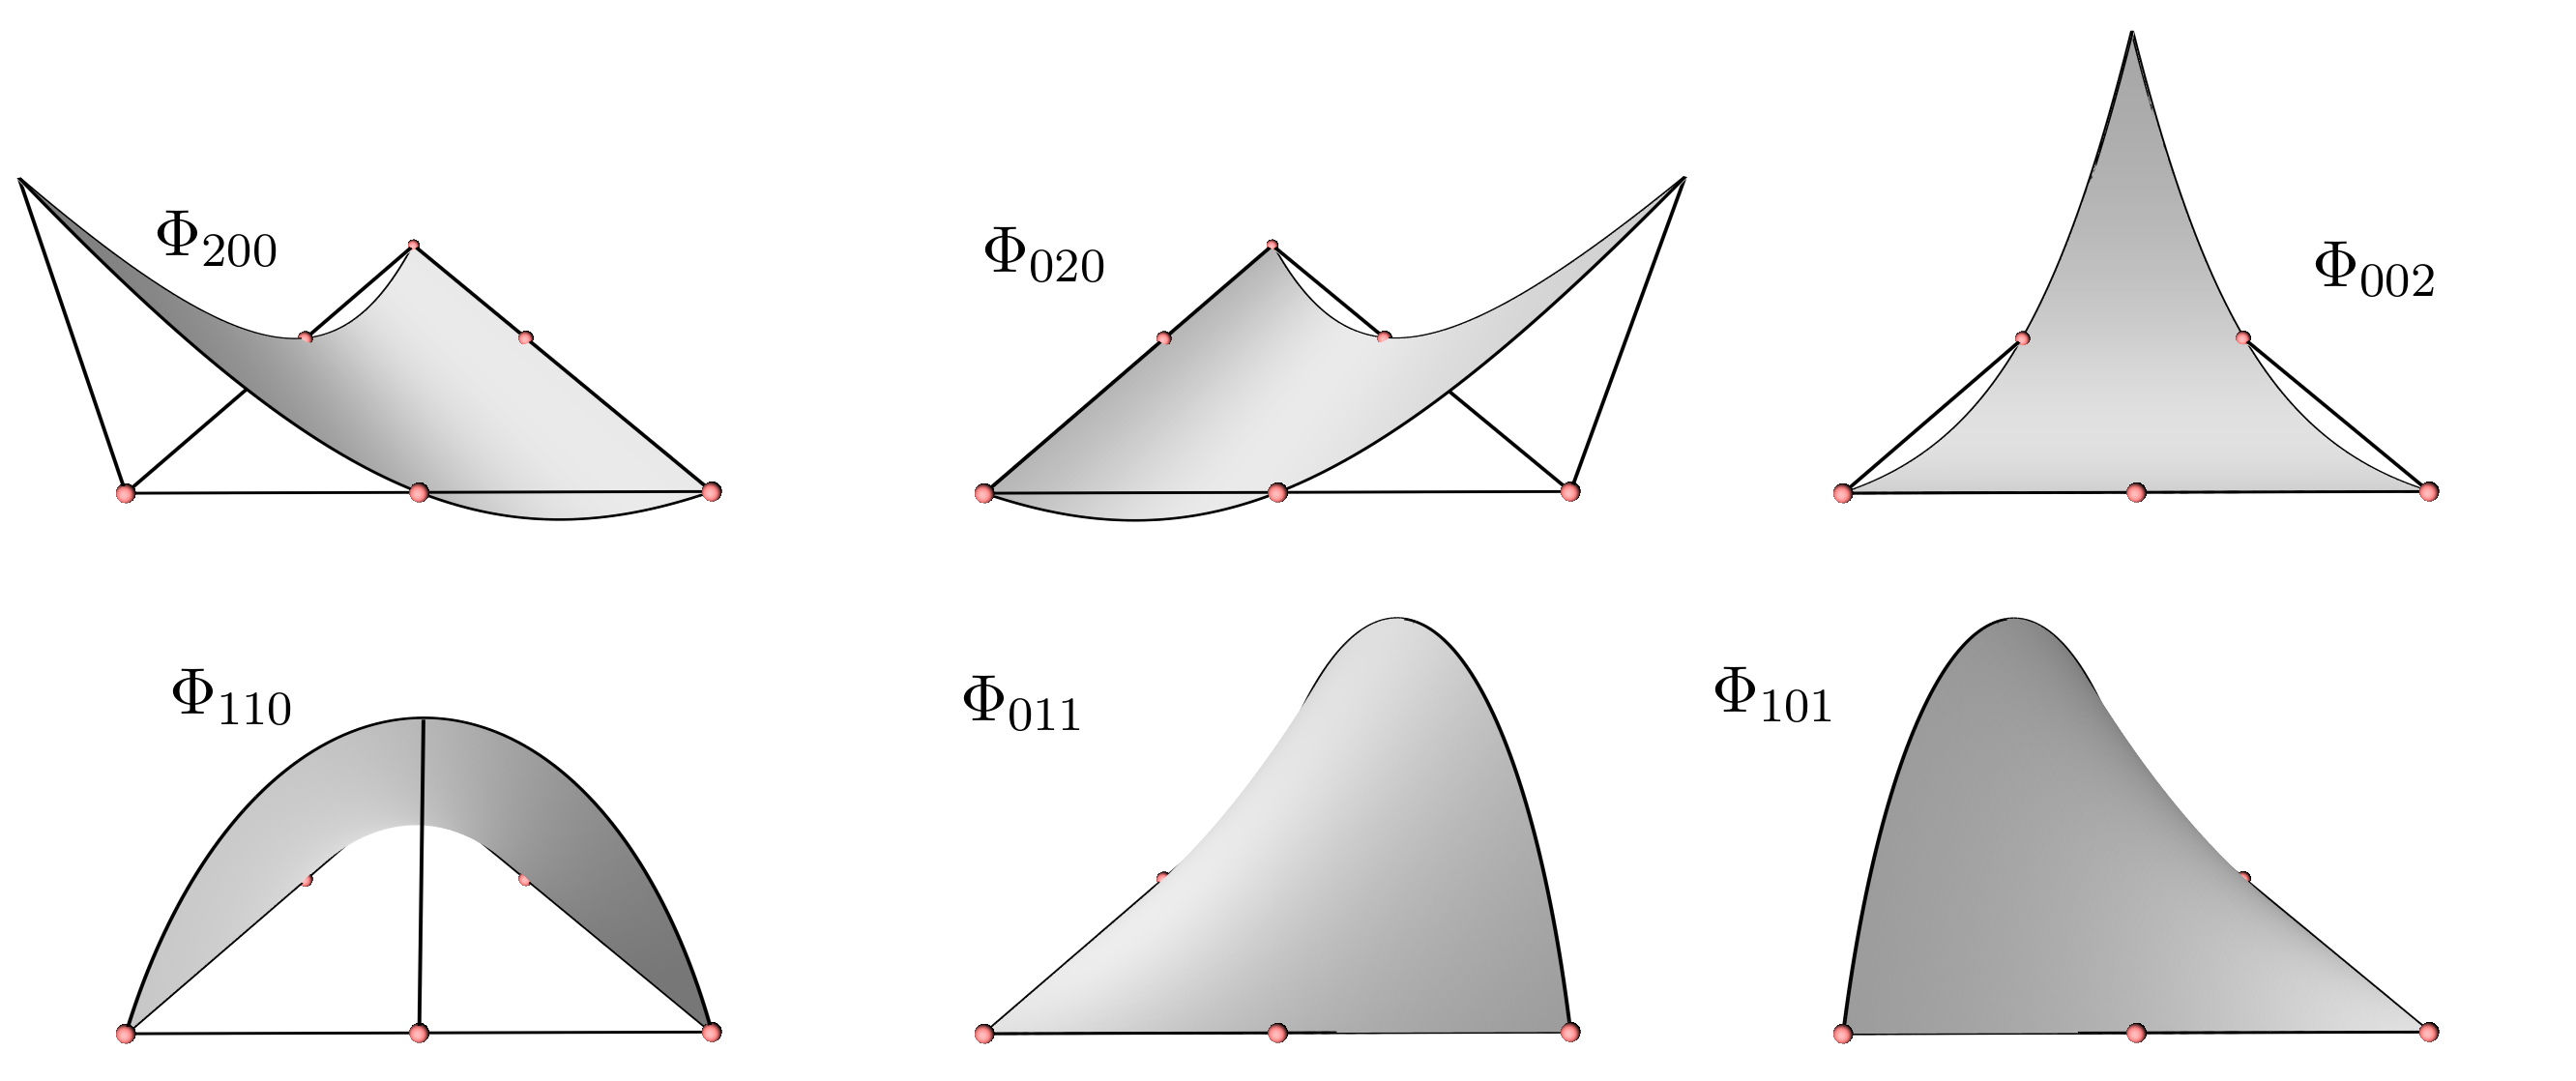
\includegraphics[width=0.86\linewidth]{figures/basis_functions/quadratic_basis_text.png}
    \end{center}
    \caption{\scriptsize
        The quadratic nodal basis functions on the triangle, where the nodes are the vertices and midpoints.
        The barycentric coordinates of the triangle vertices (from the lower-left then anticlockwise) are $(x,y,z) = (1,0,0),(0,1,0),(0,0,1)$.
    }
    \label{quadratic_basis}
\end{figure}

% Introducing some convenient notation for the piecewise quadratic basis functions,
% we refer to the basis functions corresponding to interior vertices by $\phi_1,\cdots,\phi_{n_I}$ ,
% the basis functions corresponding to boundary vertices by $\phi_1^\Gamma,\cdots,\phi_{n_\Gamma}^\Gamma$,
% and the basis function corresponding to the midpoint of adjacent vertices $i$ and $j$ by $\phi_{ij}$ and $\phi^\Gamma_{ij}$
% , respectively in the interior and on the boundary.

As the linear functions on the triangle, with incident nodes identified, implicitly defined hat functions,
so do these quadratic functions on the triangle.
We get two classes of global basis functions, formed by stitching together incident nodal basis functions:
those associated to a vertex, and those associated to a midpoint. Examples of these basis functions are displayed in figure
\ref{quadratic_basis_global}.
\begin{figure}[H]
    \begin{center}
        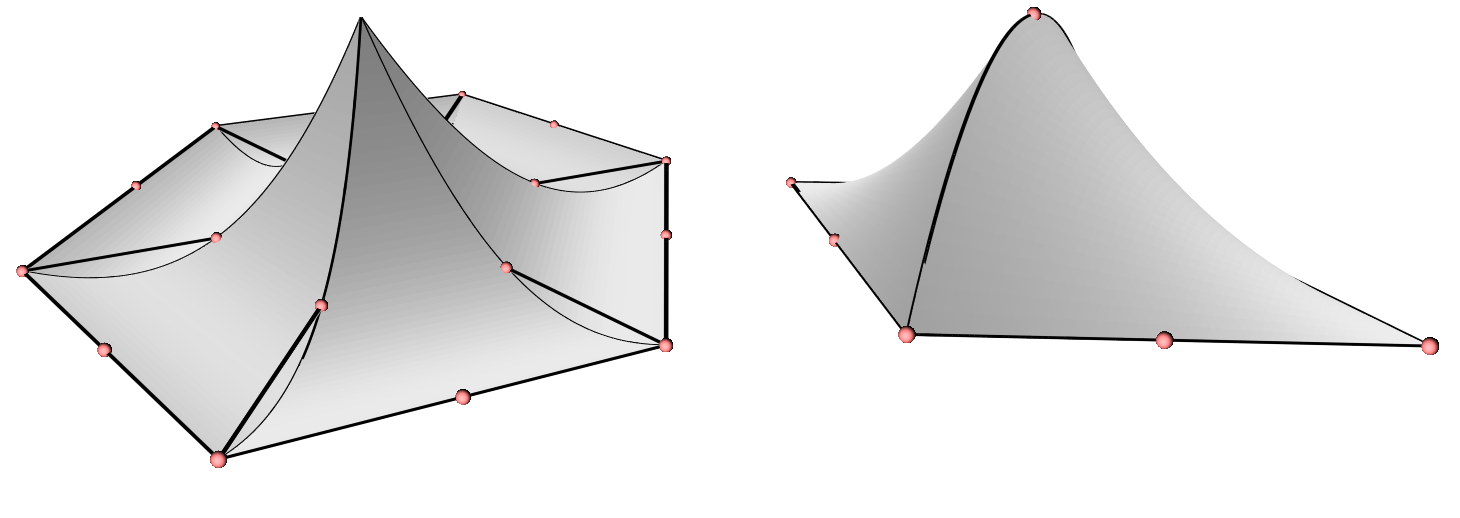
\includegraphics[width=0.8\linewidth]{figures/basis_functions/quadratic_basis_global.png}
    \end{center}
    \caption{\scriptsize
        Left: The global piecewise quadratic basis function determined by an interior vertex node, with 6 incident triangles.
        Right: The global piecewise quadratic basis function determined by an interior midpoint node.
    }
    \label{quadratic_basis_global}
\end{figure}
Much like how hat functions combine to give a piecewise linear continuous interpolation of any function, we now get
a piecewise quadratic continuous interpolation, simply by combining the basis functions by the function evaluated
at each nodal point. Example interpolations are shown in figure
\ref{quadratic_approx}.

\begin{figure}[H]
    \begin{center}
        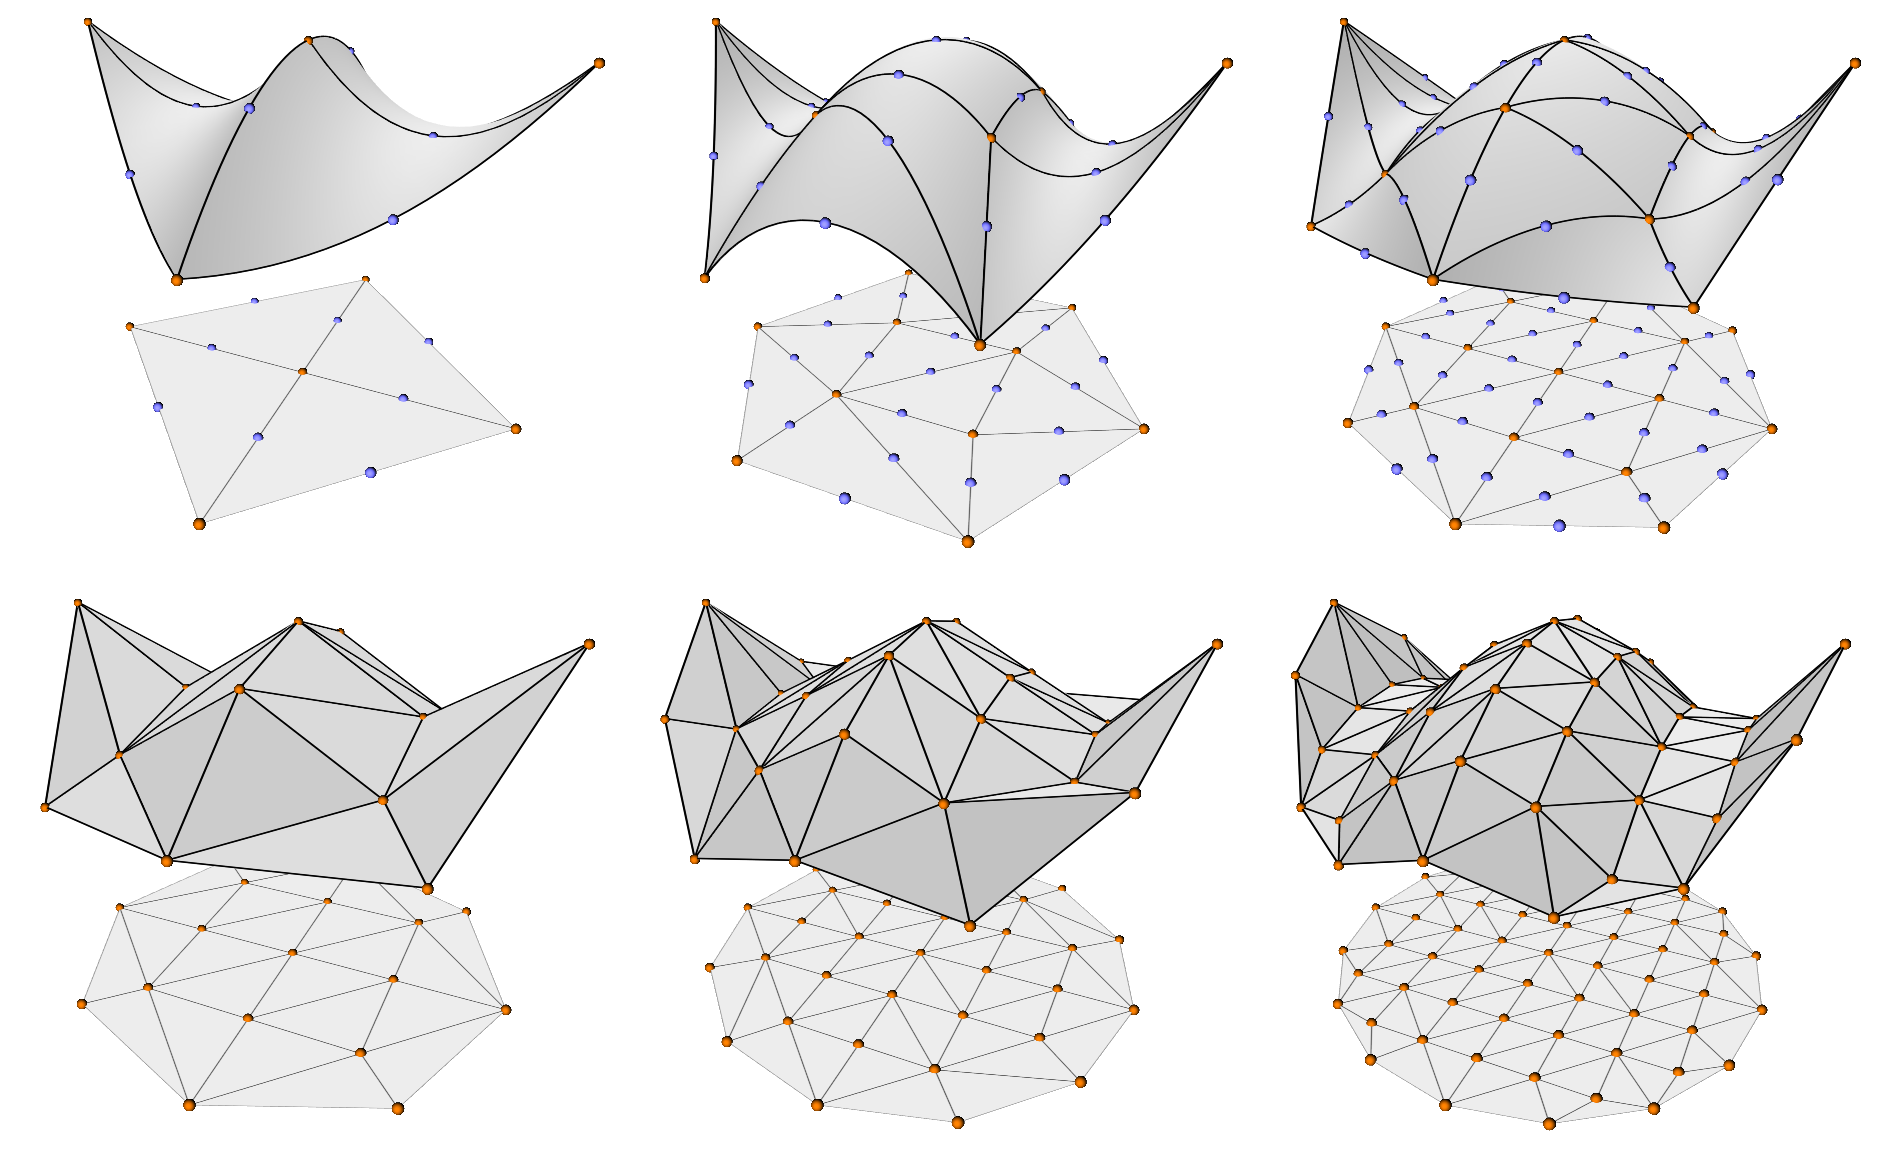
\includegraphics[width=1\linewidth]{figures/quadratic_approx/collage_1.png}
    \end{center}
    \caption{
        Interpolations of $f(x,y) = \frac{1}{2}(x^2 - y^2)+1.23 + \frac{3}{10}\cos(4x)$
        on the unit circle (with linear boundary approximation).
        First row: Piecewise quadratic interpolations of $f$.
        Second row: Piecewise linear interpolations of $f$.
        The adjacent quadratic and linear interpolations have roughly the same number of sample points ---
        the trade-off is between the number of triangles and the order of the basis functions.
    }
    \label{quadratic_approx}
\end{figure}
\subsubsection{The linear system}


\subsection{Computing the linear system for the piecewise quadratic scheme}
In section \ref{fem_closed_form} we derived the expressions needed to form the linear system for the piecewise linear scheme.
With the nodal basis functions expressed in coordinates of a reference triangle $\reftri$,
by performing a change of variables we can compute closed form expressions for the integrals restricted to each triangle.
This process is the same in the quadratic case, although it becomes more tedious.
Thankfully, this process can be automated by using an algebraic computing language --- I have used the Python library SymPy
\cite{sympy}. Listing \ref{sympy_quadratic} displays Python code which has been used to compute coefficients.
The function $\textbf{integrate\_gradients}(a,b,c, i,j,k)$ computes a symbolic definite integral,
\begin{equation}
     \int_\reftri (K\nabla\Phi^\reftri_{abc})\cdot(K\nabla\Phi^\reftri_{ijk})\,d\hat{x}
    = \int_{x=0}^{x=1}\int_{y=0}^{y=1-x} (K\nabla\Phi^\reftri_{abc})\cdot(K\nabla\Phi^\reftri_{ijk})\,dy\,dx,
\end{equation}
where $\Phi^\reftri_{abc}$ is the nodal basis function $\Phi_{abc}$ in reference triangle coordinates, with $z$ replaced by $1-x-y$.
As a rough outline, the resulting matrix assembly algorithm (for constructing $A$ and $\hat{f}$), like in the pseudocode \ref{alg:assembly},
simply
\begin{itemize}
    \item iterates over each trial basis function $\psi \in \Psi$,
    \item determines the basis functions $\phi^* \in \Phi^*$ which have domain overlapping $\psi$'s domain (by some mesh traversal),
    \item splits the domain of integration into triangles (where the restricted basis functions are quadratic --- previously they were linear),
    \item computes the integrals in closed form on this triangle (where these integrals could be derived using computer algebra),
    \item updates the matrix and RHS values, depending on whether $\phi^*$'s node is on the boundary or not.
\end{itemize}
The new matrix assembly algorithm is given in listing \ref{alg:quadratic_assembly}.
The fully expanded algorithm, with mesh traversals and closed form integrals hard-coded, is becoming nigh unreadable.
Clearly there is a simple coherent structure underlying all of these steps. We could easily generalise to piecewise cubics
by having $10 = 1 + 2 + 3 + 4$ nodes per triangle --- just find a nodal basis for cubics on a reference triangle,
and plug them into the same Python script \ref{sympy_quadratic} to derive coefficients of closed form integrals (which, again,
will be in terms of dot products between $K_1$, $K_2$, and $K_3$). We then would need to write out the whole mesh traversal
and index manipulations required, in order to implement what conceptually is a trivial increase of order from $2$ to $3$.
This process (the derivation and implementation of a finite element algorithm) is clearly a good candidate for automation.

\subsection{The resulting matrix assembly algorithm}
\subsection{The resulting finite element algorithm}
\subsection{Validation and results}

\begin{figure}
\begin{mintedbox}[mathescape=true]{python}
import sympy as sym

# Helper function to convert a barycentric index to an index into
# a flat array.
def barycentric_index_to_linear(i,j,k):
    assert(i+j+k == 2)
    ...

# Define algebraic symbols for the variables.
x,y,z = sym.symbols("x y z")

# The reference triangle has vertices $v,v^\pr,v^\ppr$.
# We define $K_1,K_2,K_3$ by
#     $K_1 = (v - v^\ppr)^\perp$,
#     $K_2 = (v^\pr - v)^\perp$,
#     $K_3 = (v^\ppr - v^\pr)^\perp$.
# $K_1$ and $K_2$ are the columns of the matrix $K$
# (which is the inverse transpose Jacobian without the constant term).
# while $K_3 = -K_1-K_2$.
K1,K2,K3 = sym.symbols("K1 K2 K3")

# Define the quadratic basis functions $\Phi_{ijk}$
# given in barycentric coordinates (x,y,z).
# The order with respect to barycentric indices is $200,020,002, 110,011,101$.
nodal_basis_functions_barycentric = [
    x*(1 - 2*y - 2*z),
    y*(1 - 2*z - 2*x),
    z*(1 - 2*x - 2*y),
    4*x*y,
    4*y*z,
    4*z*x
]
# Map the nodal basis functions to the reference triangle
# by substituting $z$ with $1-x-y$.
# These remapped basis functions will be denoted by $\Phi_{ijk}^\reftri$.
nodal_basis_functions = [p.subs(z,1-x-y).expand() for p in nodal_basis_functions_barycentric]
# Compute the gradients $\nabla\Phi_{ijk}^\reftri$.
nodal_basis_gradients = [(sym.diff(p, x), sym.diff(p, y)) for p in nodal_basis_functions]

# Provide a function to compute the integral
#     $\int_\reftri (K\nabla\Phi^\reftri_{abc})\cdot(K\nabla\Phi^\reftri_{ijk})\,d\hat{x}$
#     $= \int_{x=0}^{x=1}\int_{y=0}^{y=1-x} (K\nabla\Phi^\reftri_{abc})\cdot(K\nabla\Phi^\reftri_{ijk})\,dy\,dx.$
def integrate_gradients(a,b,c, i,j,k):
    grad1 = nodal_basis_gradients[barycentric_index_to_linear(a,b,c)]
    grad2 = nodal_basis_gradients[barycentric_index_to_linear(i,j,k)]
    f = (K1*grad1[0] + K2*grad1[1])*(K1*grad2[0] + K2*grad2[1])
    f_dy = sym.integrate(f, (y, 0,1-x))
    f_dy_dx = sym.integrate(f_dy, (x, 0,1))
    # Print the result.
    print("{}{}{},{}{}{}:".format(a,b,c,i,j,k), f_dy_dx.simplify().subs(-K1-K2,K3))
\end{mintedbox}
\caption{
    Python code to compute the closed form expressions required when forming the linear system.
    This code uses the SymPy library \cite{sympy}.
}
\label{sympy_quadratic}
\end{figure}





\newpage
\begin{algorithm}\label{alg:quadratic_assembly}
\tiny

% https://tex.stackexchange.com/questions/64204/mutliple-inputs-with-line-breaking
\newcommand\mydata[1]{%
  \settowidth\mylen{\KwData{}}%
  \setlength\hangindent{\mylen}%
  \hspace*{\mylen}#1\\}

\SetKwProg{Fn}{Routine}{\string:}{}
\SetKwProg{Def}{Define function}{\string:}{}
\Fn{Poisson\_Quadratic\_FEM\_Matrix\_Assembly}{
    \SetAlgoLined
    \KwData{Domain $\Omega$ with boundary $\Gamma$.}
    \mydata{Heat source function $g : \Omega\rightarrow \mathbb{R}$.}
    \mydata{Dirichlet boundary function $h_\Gamma : \Gamma \rightarrow \mathbb{R}$.}
    \mydata{Triangulation of $\Omega$ consisting of:}
    \mydata{\qquad Interior vertices $p_1,\cdots,p_n$.}
    \mydata{\qquad Boundary vertices $p^\Gamma_1,\cdots,p^\Gamma_{n_\Gamma}$.}
    \mydata{\qquad Interior edges $e_1,\cdots,e_m$.}
    \mydata{\qquad Boundary edges $e^\Gamma_1,\cdots,e^\Gamma_{m_\Gamma}$.}
    \mydata{\qquad Triangles $T_1,\cdots,T_{n_T}$.}
    \KwResult{
        The coefficients $(A, \hat{f})$ of the system $A\hat{h} = \hat{f}$ \eqref{poisson_matrix_equation},
        which can be solved by the caller for $\hat{h}$ in order to reconstruct
        an approximate solution $\tilde{h}:\Omega\rightarrow\mathbb{R}$ of the boundary value problem \eqref{poisson_dirichlet_problem},\\
        \qquad\qquad\qquad\qquad $-\Delta h = g$, $\left.h\right|_\Gamma = h_\Gamma$.
    }
    $N \leftarrow n + m$\;
    $A \leftarrow \text{$N\times N$ zero matrix}$\;
    $\hat{f} \leftarrow \text{length $N$ zero vector}$\;
    \For{$j = 1,\cdots,n$}{
        Let $v$ denote the interior vertex $p_j$.\\
        Let $v_1,\cdots,v_k$ denote the vertices adjacent to $v$.\\
        Let $T^v_1,\cdots,T^v_k$ denote the triangles adjacent to $v$.\\
        (Triangle $T^v_t$ joins vertices $v,v_t,v_{t+1}$.)\\
        Let $e^v_1,\cdots,e^v_k$ denote the edges from $v$ to each $v_1,\cdots,v_k$.\\
        \For{$t = 1,\cdots, k$}{
            $C \leftarrow \frac{1}{4\text{Area}(T^v_t)}$\;
            $K_1 \leftarrow (v - v_{t+1})^\perp, \quad
            K_2 \leftarrow (v_t - v)^\perp, \quad
            K_3 \leftarrow (v_{t+1} - v_t)^\perp$\;
            $A[j,j] \leftarrow A[j,j] + \frac{1}{2}C\norm{K_3}^2$\;
            \uIf{$v_t$ is on the boundary}{
                $\hat{f}[I(v_t)] \leftarrow \hat{f}[I(v_t)] + \frac{1}{6}h_\Gamma(v_t)C K_1\cdot K_3$\;
            }
            \Else{
                $A[j, I(v_t)] \leftarrow A[j, I(v_t)] - \frac{1}{6}C K_1\cdot K_3$\;
            }
            \uIf{$v_{t+1}$ is on the boundary}{
                $\hat{f}[I(v_{t+1})] \leftarrow \hat{f}[I(v_{t+1})] + \frac{1}{6}h_\Gamma(v_{t+1})C K_2\cdot K_3$\;
            }
            \Else{
                $A[j, I(v_{t+1})] \leftarrow A[j, I(v_{t+1})] - \frac{1}{6}C K_2\cdot K_3$\;
            }
            
            $A[j, I(e^v_t)] \leftarrow A[j, I(e^v_t)] + \frac{2}{3} C K_1\cdot K_3$\;
            $A[j, I(e^v_{t+1})] \leftarrow A[j, I(e^v_{t+1})] + \frac{2}{3} C K_2\cdot K_3$\;
        }
    }
    \For{$j = 1,\cdots,m$}{
        Let $e$ denote the interior edge $e_j$.\\
        Denote by $T_0^e$ and $T_1^e$ the two triangles incident to $e$.\\
        \For{$t = 0,1$}{
            $C \leftarrow \frac{1}{4\text{Area}(T_t^e)}$\;
            Let $v,v^\pr,v^\ppr$ be the anticlockwise vertices of $T^e_t$, where $v$ is the vertex opposite to $e$.\\
            Let $e^\pr$ and $e^\ppr$ be the edges from $v$ to $v^\pr$ and from $v$ to $v^\ppr$, respectively.\\
            $K_1 \leftarrow (v - v^\ppr)^\perp,\quad
                K_2 \leftarrow (v^\pr - v)^\perp,\quad
                K_3 \leftarrow (v^\ppr - v^\pr)^\perp$\;

            % // printf("self midpoint\n");
            % double val = 0.;
            % // 110, 110
            % // val = 4.*C/3. * (K3.dot(K3) - K1.dot(K2));
            % val = 4.*C/3. * (K1.dot(K1) + K1.dot(K2) + K2.dot(K2));
            % add_entry(num_interior_vertices + midpoint_index, num_interior_vertices + midpoint_index, val);
            $A[n+j, n+j] \leftarrow A[n+j, n+j] + \frac{4}{3} C (\norm{K_3} - K_1\cdot K_2)$\;

            % // printf("boundary midpoints\n");
            % // 110, 011
            % val = 4.*C/3. * (K1.dot(K3));
            % if (midpoint_vpp.on_boundary()) {
            %     double bv = dirichlet_boundary_function(midpoint_vpp_pos.x(), midpoint_vpp_pos.z());
            %     rhs[num_interior_vertices + midpoint_index] -= bv * val;
            % } else {
            %     add_entry(num_interior_vertices + midpoint_index, num_interior_vertices + midpoint_vpp_index, val);
            % }
            \uIf{$e^\ppr$ is on the boundary}{
                $b[n+j] \leftarrow b[n+j] - \frac{4}{3} h_\Gamma(e^\ppr \text{midpoint}) C K_1\cdot K_3$\;
            } \Else {
                $A[n+j, I(e^\ppr)] \leftarrow A[n+j, I(e^\ppr)] + \frac{4}{3} C K_1\cdot K_3$\;
            }
            % // 110, 101
            % val = 4.*C/3. * (K2.dot(K3));
            % if (midpoint_vp.on_boundary()) {
            %     double bv = dirichlet_boundary_function(midpoint_vp_pos.x(), midpoint_vp_pos.z());
            %     rhs[num_interior_vertices + midpoint_index] -= bv * val;
            % } else {
            %     add_entry(num_interior_vertices + midpoint_index, num_interior_vertices + midpoint_vp_index, val);
            % }
            \uIf{$e^\pr$ is on the boundary}{
                $b[n+j] \leftarrow b[n+j] - \frac{4}{3} h_\Gamma(e^\pr \text{midpoint}) C K_2\cdot K_3$\;
            } \Else {
                $A[n+j, I(e^\pr)] \leftarrow A[n+j, I(e^\pr)] + \frac{4}{3} C K_2\cdot K_3$\;
            }

            % // printf("vertices\n");
            % // 110, 200
            % val = 2.*C/3. * (K1.dot(K2));
            % if (vp.on_boundary()) {
            %     double bv = dirichlet_boundary_function(vp_pos.x(), vp_pos.z());
            %     rhs[num_interior_vertices + midpoint_index] -= bv * val;
            % } else {
            %     add_entry(num_interior_vertices + midpoint_index, vp_index, val);
            % }
            \uIf{$v^\pr$ is on the boundary}{
                $b[n+j] \leftarrow b[n+j] - \frac{2}{3} h_\Gamma(v^\pr) C K_1\cdot K_2$\;
            } \Else {
                $A[n+j, I(v^\pr)] \leftarrow A[n+j, I(v^\pr)] + \frac{2}{3} C K_1\cdot K_2$\;
            }

            % // 110, 020
            % if (vpp.on_boundary()) {
            %     double bv = dirichlet_boundary_function(vpp_pos.x(), vpp_pos.z());
            %     rhs[num_interior_vertices + midpoint_index] -= bv * val;
            % } else {
            %     add_entry(num_interior_vertices + midpoint_index, vpp_index, val);
            % }
            \uIf{$v^\ppr$ is on the boundary}{
                $b[n+j] \leftarrow b[n+j] - \frac{2}{3} h_\Gamma(v^\ppr) C K_1\cdot K_2$\;
            } \Else {
                $A[n+j, I(v^\ppr)] \leftarrow A[n+j, I(v^\ppr)] + \frac{2}{3} C K_1\cdot K_2$\;
            }
        }
    }
    \Return{$(A, \hat{f})$}\;
    % Solve $A\hat{h} = b$ for $\hat{h} = (h_1,\cdots,h_n)^T$\;
    % $\tilde{h} \leftarrow \sum_{j=1}^n h_j\text{Hat}(p_j) + \sum_{j=1}^{n_\Gamma} h_\Gamma(p_j^\Gamma)\text{Hat}(p_j^\Gamma)$\;
    % \Return{$\tilde{h}$}\;
}
    \caption{Text}
\end{algorithm}
\newpage

\begin{figure}[H]
    \begin{center}
        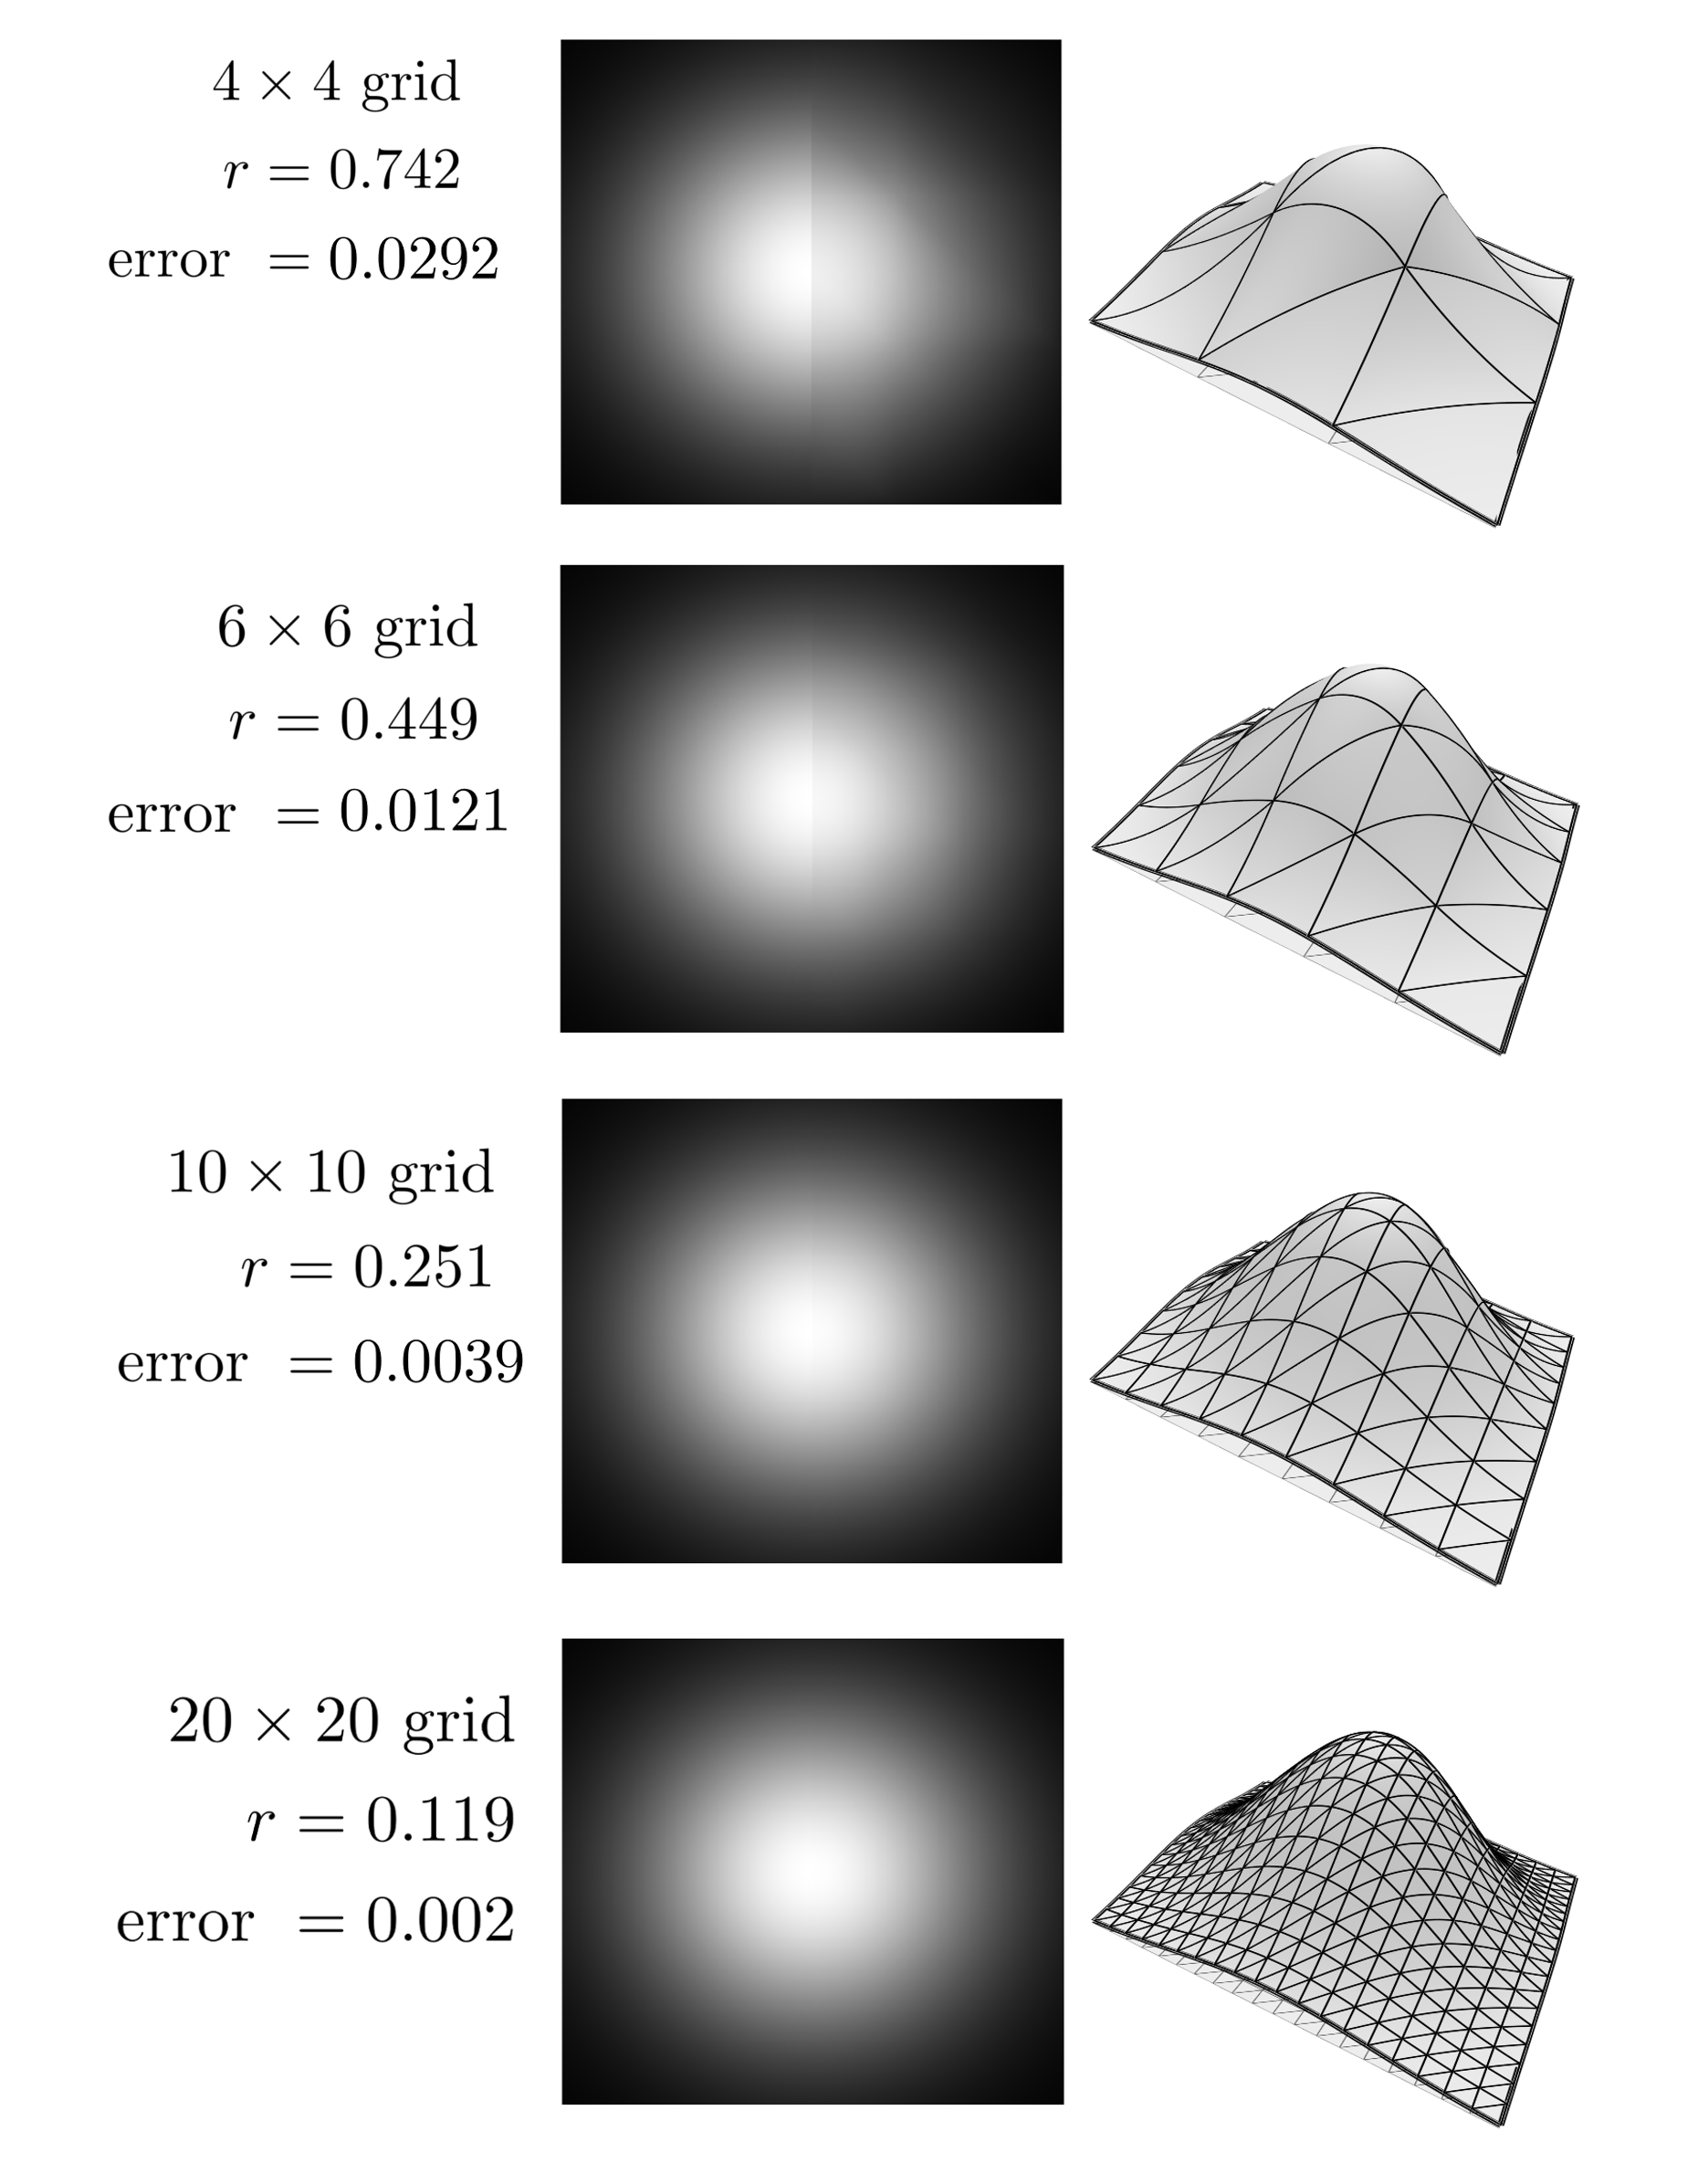
\includegraphics[width=1\linewidth]{figures/quadratic_error/quadratic_error.png}
    \end{center}
    \caption{
        Approximate solutions to the test problem \eqref{fvm_test_equation_2} with varying $r$.
        The middle squares contain plots of the exact solution (on the left rectangle), and the approximate solution (on the right rectangle).
        Black is $h = 0$, and white is $h = 1$.
        On the right, a 3D view of the solution and mesh is shown.
    }
    \label{quadratic_fem_error_page}
\end{figure}

